\documentclass[12font]{article}
\title{\textbf{Loopy Genuine Multipartite Entanglement in the Kitaev Model}}
\author{Chen-Chih Wang  }
\date{\textit{Department of Physics, National Tsing Hua University, Hsinchu 30013, Taiwan} \\ (Dated: \today)}
\usepackage[margin=2cm]{geometry}
%\usepackage[fleqn]{amsmath}
%\usepackage{CJK,amsmath}
\usepackage{amsfonts,amssymb}
\usepackage{amsmath}
\numberwithin{equation}{section}    % numbering equations by their section
\usepackage{fancyhdr}
%\pagestyle{fancy}
\usepackage{textcomp}
\usepackage{graphicx}
\usepackage{float}
\usepackage{color}
\usepackage{tikz}
\usepackage{multicol}
\usepackage{threeparttable}
\usepackage{amsthm}
\usepackage{mathtools}
\usepackage{hyperref}
\urlstyle{same}
\usepackage{caption}
\usepackage{subcaption}
\usepackage{dsfont}
\usepackage{qcircuit} % quantum circuit

\usepackage{algorithm}
\usepackage{algpseudocode}

\newtheorem{theorem}{Theorem}[section]
\theoremstyle{definition}
\newtheorem{definition}{Definition}[section]
\newtheorem{lemma}[theorem]{Lemma}
\newtheorem{corollary}{Corollary}[theorem]
\newtheorem{proposition}[theorem]{Proposition}

\hypersetup{
    colorlinks=true,
    linkcolor=blue,
    filecolor=magenta,      
    urlcolor=blue,
    pdftitle={Overleaf Example},
    pdfpagemode=FullScreen,
    }
\usepackage[numbers,sort&compress]{natbib}

\newcommand{\vac}{\mrm{vac}}
\newcommand{\Bra}[1]{\left\langle #1 \right|}
\newcommand{\Ket}[1]{\left| #1 \right\rangle}
\newcommand{\bra}[1]{\langle #1 |}
\newcommand{\ket}[1]{| #1 \rangle}
\newcommand{\anglelr}[1]{\langle #1 \rangle}
\newcommand{\Anglelr}[1]{\left\langle #1 \right\rangle}
\newcommand{\braket}[2]{\langle #1 | #2 \rangle}
\newcommand{\Bbraket}[2]{\left\langle #1 \right|\left. #2 \right\rangle}
\newcommand{\dif}[1]{\frac{\mathrm{d}}{\mathrm{d}#1}}
\newcommand{\diff}[2]{\frac{\mathrm{d}#1}{\mathrm{d}#2}}
\newcommand{\gd}{\boldsymbol{\nabla}}
\newcommand{\dive}{\boldsymbol{\nabla}\cdot}
\newcommand{\curl}{\boldsymbol{\nabla}\times}
\newcommand{\lrno}[1]{\left.#1\right.}
\newcommand{\lr}[1]{\left(  #1  \right)}
\newcommand{\lrm}[1]{\left[  #1  \right]}
\newcommand{\lrg}[1]{\left\{  #1  \right\}}
\newcommand{\abs}[1]{\left|  #1  \right|}
\newcommand{\de}{\partial}
\newcommand{\pdif}[1]{\frac{\partial}{\partial#1}}
\newcommand{\pdiff}[2]{\frac{\partial#1}{\partial#2}}
\newcommand{\mrm}[1]{\mathrm{#1}}
\newcommand{\bo}[1]{\mathbf{#1}}
\newcommand{\bog}[1]{\boldsymbol{#1}}
\newcommand{\vint}[3]{\int_{#1}#2\cdot\mathrm{d}\mathbf{#3}}
\newcommand{\voint}[3]{\oint_{#1}#2\cdot\mathrm{d}\mathbf{#3}}
\newcommand{\Vint}{\int\mrm{d}^3\bo{r}'}
\newcommand{\rr}{\mathbf{r} - \mathbf{r}'}
\newcommand{\arr}{\left|\mathbf{r} - \mathbf{r}'\right|}
\newcommand{\nx}{\hat{\bo{n}}_1}
\newcommand{\ny}{\hat{\bo{n}}_2}
\newcommand{\alert}[1]{{\color{red}#1}}
\newcommand{\alertV}[1]{{\color{violet}#1}}
\newcommand{\Tr}{\mrm{Tr}}
\newcommand{\tr}{\mrm{tr}}
\newcommand{\norm}[1]{\left\lVert#1\right\rVert}
\newcommand{\tcor}[2]{\langle -ic_{#1}c_{#2} \rangle_M}

\newcommand{\arrequ}[1]{\begin{aligned}#1\end{aligned}}

\newcommand{\Qcirc}[1]{\begin{minipage}[h]{0.7cm}
	\vspace{0pt}
	\Qcircuit @C=1em @R=.7em {#1}
   \end{minipage}}
\newcommand{\dimer}[2]{\sigma_{#1}^{\alpha_{#1#2}}\sigma_{#2}^{\alpha_{#1#2}}}

\begin{document}
\maketitle
\renewcommand\qedsymbol{$\blacksquare$}



\fontsize{12pt}{16pt}\selectfont

\begin{abstract}
    In this note, we discuss how to compute multi-spin correlation functions in a finite-size Kitaev model, which only contains four distinct plaquettes. These correlation functions are crucial in constructing the density matrix of the Kitaev ground state.
\end{abstract}

\tableofcontents

\section{Foundations}

\subsection{Correlation Functions}
As mentioned in our work~\cite{wang2026exactorganizationdensitymatrices}, at the ground state, the multi-spin correlation function of the Kitaev model is finite if and only if it can be written in the form of a string. Therefore, we only need to discuss the following form of the correlation function
\[
\Anglelr{
    \prod_{\anglelr{ij}\in\mathfrak{D}}
    \dimer{i}{j}
}
\]
This kind of correlation function can be exactly evaluated in the Majorana representation. Substituting the transformation 
\[
\dimer{i}{j} \to i b^{\alpha_{ij}}_i c_i  i b^{\alpha_{ij}}_j c_j = \hat{u}_{ij} ic_jc_i
\]
into the correlation function and taking the trivial gauge, we have
\[
\Anglelr{
    \prod_{\anglelr{ij}\in\mathfrak{D}}
    \dimer{i}{j}
}
=
\Anglelr{
    \prod_{\anglelr{ij}\in\mathfrak{D}}
    (-i) c_ic_j
}_M
\]

\subsection{Minimal Size for Non-trivial Topology}
For numerical efficiency, we tend to choose the smallest possible system. However, the system must still be sufficiently large such that the topological order still exists. A requirement for this is that the ground state manifold should possess four independent topological sectors generated by global Wilson loops if the geometry of the system is a torus.

We start from the Wen plaquette model. There are two requirements for a Wen plaquette system to possess four topologically degenerate ground states:
\begin{itemize}
    \item The lattice must contain an even number of rows or columns in both the horizontal and vertical directions.
    
    \item A global Wilson loop cannot be generated or destroyed by local plaquette operators.
\end{itemize}
The physical meaning of the first requirement is to preserve the checkerboard pattern of the lattice. If there are adjacent plaquettes (cells) that are of the same type (black or white, in a checkerboard sense), then the two types of plaquettes become identical, and the original two different Wilson loops become the same. This breakdown of the checkerboard pattern reduces the original fourfold topological ground state degeneracy down to twofold, which is not adequate to describe the physics of a toric code system.

According to the two requirements, \textbf{the smallest possible topologically non-trivial Wen plaquette model contains eight ($8 = 2\times 4$) distinct plaquettes and eight sites}. A $2\times 2$ checkerboard is not adequate for the system to have four topological sectors since it violates the second requirement\footnote{The \textit{global Wilson loop} is identical to a plaquette operator}. 

\begin{figure}
    \centering
    (a)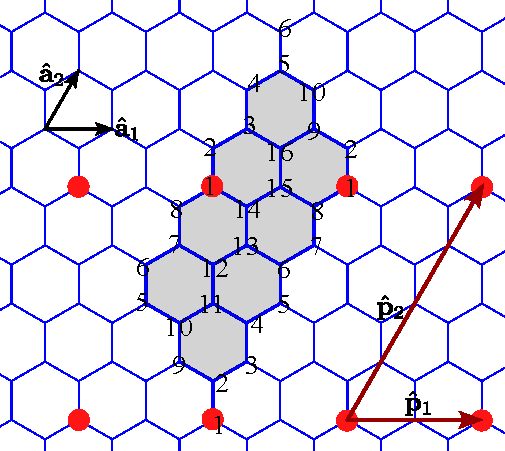
\includegraphics[height=0.15\textheight]{figures/minimal-system.pdf}
    \hspace{5mm}
    (b)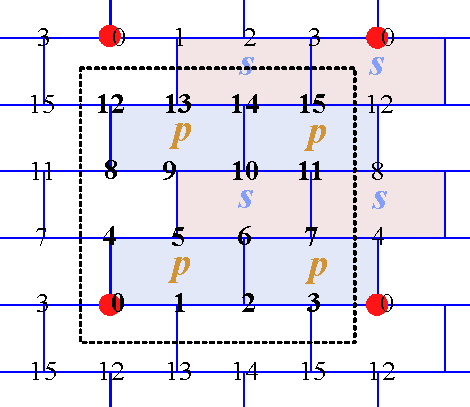
\includegraphics[height=0.15\textheight]{figures/minimal-system_brick-wall.pdf}
    \hspace{5mm}
    (c)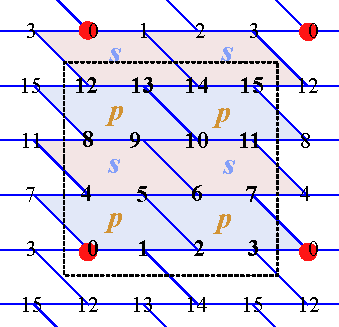
\includegraphics[height=0.15\textheight]{figures/minimal-system_brick-wall_diagonal.pdf}
    \caption{(a) The smallest topologically non-trivial system consists of 8 unit cells, which is equivalent to 16 spins. The two vectors that define the periodic boundary condition are $\hat{\bo{p}}_1 = 2\hat{\bo{a}}_1$ and $\hat{\bo{p}}_2 = 4\hat{\bo{a}}_2$, respectively. (b) For numerical simplicity, the honeycomb lattice is rearranged into a brick-wall geometry, and the spins are relabeled according to their Euclidean coordinates in the lattice. In both figures, red dots indicate identical lattice sites. (c) An equivalent choice.}
    \label{fig:lattice}
\end{figure}
\section{Finite-Size Correlation}
We only have to focus on the two-point correlation functions. Here we set that the system satisfies the \textbf{periodic boundary condition}, which is characterized by two independent vectors, $\hat{\bo{p}}_1 = 2\hat{\bo{a}}_1$ and $\hat{\bo{p}}_2 = 4\hat{\bo{a}}_2$, as illustrated in Fig.\ref{fig:lattice}.a. The geometry adopted here follows the one illustrated in Ref.~\cite{Pedrocchi-Chesi-Loss_2011}

\subsection{Momentum States in Finite Systems}
For slave fermions in the parton construction, the boundary condition of the system could be periodic (PBC) or anti-periodic (APBC), depending on which topological sector we choose~\cite{Kou-Levin-Wen_2008}. Here, we only consider the PBC in both the horizontal and vertical directions. 
\begin{equation}\label{eq:PBC}
    f_{\sigma\mu\bo{x}} = f_{\sigma\mu,(\bo{x} + \hat{\bo{p}}_1)} = f_{\sigma\mu,(\bo{x} + \hat{\bo{p}}_2)}
\end{equation}
To determine the allowed momentum states, we first Fourier transform the fermions as follows
\[
f_{\sigma\mu\bo{x}} = \frac{1}{\sqrt{N/2}}\sum_{\bo{k}} e^{i\bo{k}\cdot\bo{x}} f_{\sigma\mu\bo{k}}
\]
With this expression, Eq.~\eqref{eq:PBC} implies that the allowed momentum $\bo{k}$ must satisfy
\begin{equation}\label{eq:condition-init}
    \left\{
    \begin{array}{lll}
        \bo{k}\cdot\hat{\bo{p}}_1 = 2n_1\pi & ; & n_1 = 0,1,\cdots,N_h-1\\
        \bo{k}\cdot\hat{\bo{p}}_2 = 2n_2\pi & ; & n_2 = 0,1,\cdots,N_v-1
    \end{array}
    \right.
\end{equation}
In our case illustrated in Fig.~\ref{fig:lattice}, $N_h=2$ and $N_v = 4$, representing the number of unit cells included in the system in the horizontal and vertical directions, respectively. Consider the unit vectors $\hat{\bo{a}}_1 = \hat{\bo{e}}_x$ and $\hat{\bo{a}}_2 = \frac{1}{2}\hat{\bo{e}}_x + \frac{\sqrt{3}}{2}\hat{\bo{e}}_y$. We can define the unit vectors in the momentum space as 
\[
\left\{
\begin{aligned}
& \hat{\bo{b}}_1 =  2\pi\hat{\bo{e}}_x - \frac{2\pi}{\sqrt{3}}\hat{\bo{e}}_y\\
& \hat{\bo{b}}_2 = \frac{4\pi}{\sqrt{3}}\hat{\bo{e}}_y
\end{aligned}
\right.
\]
such that $\hat{\bo{a}}_i\cdot\hat{\bo{b}}_j = 2\pi \delta_{ij}$. With these basis vectors, the allowed momentum states are
\begin{equation}\label{eq:allowed-momentum}
    \bo{k} = \frac{n_1}{2}\hat{\bo{b}}_1 + \frac{n_2}{4}\hat{\bo{b}}_2 \quad ; \quad n_1=0,1 \quad,\quad n_2=0,1,2,3
\end{equation}

In general, if the relation between two representations $\bo{k} = k_x\hat{\bo{e}}_x + k_y\hat{\bo{e}}_y = k_1\hat{\bo{b}}_1 + k_2\hat{\bo{b}}_2$ is
\[
\begin{array}{ccc}
    \left\{
    \begin{aligned}
        & k_x = 2\pi k_1 \\
        & k_y = \frac{2\pi}{\sqrt{3}}\lr{-k_1 + 2k_2}
    \end{aligned}
    \right.
    &  
    ,
    &
    \left\{
    \begin{aligned}
        & k_1 = \frac{1}{2\pi} k_x \\
        & k_2 = \frac{1}{4\pi}\lr{k_x + \sqrt{3}k_y}
    \end{aligned}
    \right.
\end{array}
\]


\subsection{Two-Points Correlation Functions}
The correlation functions can be calculated more easily in the normal fermion language. As defined in the appendix, the $c$-Majorana fermions can be written in terms of $\gamma$-fermions,
\[
\left\{
\begin{aligned}
& c_{\bo{x}A} =  \gamma^\dagger_{\bo{x}} + \gamma_{\bo{x}} = \frac{1}{\sqrt{N/2}}\sum_{\bo{k}}\lr{\gamma^\dagger_k e^{-ik\bo{x}} + \gamma_{\bo{k}} e^{ik\bo{x}}} \\
& c_{\bo{x}B} = i\lr{\gamma^\dagger_{\bo{x}} - \gamma_{\bo{x}}} = \frac{i}{\sqrt{N/2}}\sum_{\bo{k}}\lr{\gamma^\dagger_k e^{-ik\bo{x}} - \gamma_{\bo{k}} e^{ik\bo{x}}}
\end{aligned}
\right.
\]
And the ground state is 
\[
\ket{\psi} = A\exp\lr{\sum_{k\in\mrm{HBZ}}g_k\gamma^\dagger_k\gamma^\dagger_{-k}}
\]
where 
\[
A = \prod_{k\in\mrm{HBZ}}\lr{1 + \abs{g_k}^2}^{-1/2}
\]
is the normalization constant. Similar to Numbu-Gor'kov Green's function, there are two types of fermion pairing, $AA(BB)$ and $AB$. Both types of correlation functions can be simplified to the problem of solving the $\gamma$-fermion correlation function as we will see later. The two $\gamma$-fermion correlation functions we have to know are $\anglelr{\gamma_{\bo{k}}\gamma_{k'}}$ and $\anglelr{\gamma^\dagger_k\gamma_{k'}}$. Their analytical forms are given as follows
\[
\left\{
\begin{aligned}
& \anglelr{\gamma^\dagger_k \gamma_{k'}} = \frac{\abs{g_k}^2}{1+\abs{g_k}^2}\delta_{kk'} = v_k^2\delta_{kk'} = \frac{1}{2}\lr{1-\frac{R_{\bo{k}}}{\abs{s_{\bo{k}}}}}\delta_{kk'}\\
& \anglelr{\gamma_{\bo{k}}\gamma_{k'}} = \frac{g_k}{1+\abs{g_k}^2}\delta_{k,-k'} = i\mrm{sgn}\lr{I_k}u_kv_k\delta_{k,-k'} = i\frac{I_k}{2\abs{s_{\bo{k}}}}\delta_{k,-k'}
\end{aligned}
\right.
\]
and the fermionic commutation relations can give other two types of correlation functions
\[
\left\{
\begin{aligned}
& \anglelr{\gamma_{\bo{k}}\gamma_{k'}^\dagger} = \delta_{kk'} - \anglelr{\gamma^\dagger_{k'}\gamma_{\bo{k}}} = u^2_k\delta_{kk'} = \frac{1}{2}\lr{1+\frac{R_{\bo{k}}}{\abs{s_{\bo{k}}}}}\delta_{kk'} \\
& \anglelr{\gamma_{\bo{k}}^\dagger\gamma_{k'}^\dagger} = \anglelr{\gamma_{k'}\gamma_{\bo{k}}}^* = -i\mrm{sgn}(I_{k'})u_{k'}v_{k'}\delta_{k',-k} = i\mrm{sgn}(I_{k})u_{k}v_{k}\delta_{k,-k'} = \anglelr{\gamma_{\bo{k}}\gamma_{k'}}
\end{aligned}
\right.
\]

Here I list the explicit expression of $s_k$, $R_k$ and $I_k$ and other relevant quantities or functions. We start from 
\[
s_k = 2\lr{J_x e^{ik\cdot \hat{\bo{n}}_1} + J_y e^{ik\cdot \hat{\bo{n}}_2} + J_z}
\]
Then, if we express the momentum state in terms of $\bo{k} = k_x\hat{\bo{e}}_x + k_y\hat{\bo{e}}_2$, then
\begin{equation}\label{eq:functions}
  \left.
  \begin{aligned}
  &\abs{s_k} = 2\lrm{J_x^2+J_y^2+J_z^2 + 2J_xJ_y\cos\lr{k_x} + 2J_xJ_z\cos\lr{\frac{1}{2}k_x+\frac{\sqrt{3}}{2}k_y} + 2J_yJ_z\cos\lr{\frac{1}{2}k_x-\frac{\sqrt{3}}{2}k_y}}^{1/2} \\
  & R_k = 2\lrm{J_x\cos\lr{\frac{1}{2}k_x+\frac{\sqrt{3}}{2}k_y} + J_y\cos\lr{\frac{1}{2}k_x-\frac{\sqrt{3}}{2}k_y} + J_z}\\
  &I_k = 2\lrm{J_x\sin\lr{\frac{1}{2}k_x+\frac{\sqrt{3}}{2}k_y} - J_y\sin\lr{\frac{1}{2}k_x-\frac{\sqrt{3}}{2}k_y}}
  \end{aligned}
  \right\}
\end{equation}
Or, expressed in terms of reciprocal basis vectors $\bo{k} = k_1\hat{\bo{b}}_1 + k_2\hat{\bo{b}}_2$, then
\begin{equation}\label{eq:functions_b}
  \left.
  \begin{aligned}
  &\abs{s_k} 
  = 
  2\lrm{
      J_x^2+J_y^2+J_z^2 + 2J_xJ_y\cos\lr{2\pi k_1} 
      + 
      2J_xJ_z\cos\lr{2\pi k_2} 
      + 
      2J_yJ_z\cos\lr{2\pi (k_1 - k_2)}
  }^{1/2} \\
  & R_k 
  = 2\lrm{
      J_x\cos\lr{2\pi k_2} 
      + 
      J_y\cos\lr{2\pi (k_1 - k_2)} 
      + 
      J_z
  }\\
  &I_k 
  = 2\lrm{
      J_x\sin\lr{2\pi k_2} 
      - 
      J_y\sin\lr{2\pi (k_1 - k_2)}
  }
  \end{aligned}
  \right\}
\end{equation}
Again, these results are general and are valid even in a finite-size system.

With these relations, we can start to compute the $c$-Majorana correlation functions. For $AA$-pairings, the correlation function is,
\begin{align*}
  \anglelr{c_{\bo{x}A}c_{\bo{x}'A}} &= \frac{1}{N/2}\sum_{\bo{k}}\lr{ \anglelr{\gamma_{\bo{k}}\gamma_{-\bo{k}}} + \anglelr{\gamma_{-\bo{k}}^\dagger\gamma^\dagger_{k}} +
  \anglelr{\gamma_{\bo{k}}\gamma_{k}^\dagger} + 
  \anglelr{\gamma_{-\bo{k}}^\dagger\gamma_{-\bo{k}}}
  }e^{i\bo{k}\cdot\lr{\bo{x}-\bo{x'}}} \\
  &= \frac{1}{N/2}\sum_{\bo{k}}\lr{1-\frac{R_{\bo{k}}}{\abs{s_{\bo{k}}}}}e^{i\bo{k}\cdot\lr{\bo{x}'-\bo{x}}} \\
  &= \frac{1}{N/2}\sum_{\bo{k}}\lr{1-\frac{R_{\bo{k}}}{\abs{s_{\bo{k}}}}}\cos\lr{\bo{k}\cdot\lr{\bo{x}'-\bo{x}}} \in \mathbb{R}
\end{align*}
The imaginary part is an odd function in the momentum space, hence it vanishes after the integration. However, this implies that the Majorana correlation function is a real number, which is impossible since
\[
\anglelr{c_ic_j}^* = \anglelr{c_jc_i} = -\anglelr{c_ic_j}
\]
which must be an imaginary number unless $i=j$. So we conclude that
\begin{equation}\label{correlationAA.e}
  \anglelr{c_{\bo{x}A}c_{\bo{x'}A}} = \anglelr{c_{\bo{x}B}c_{\bo{x'}B}} = \delta_{\bo{x}\bo{x'}}
\end{equation}


As for $AB$-pairings, a similar calculation gives
\begin{align*}
  \anglelr{c_{\bo{x}A}c_{\bo{x}'B}} &= \frac{i}{N/2}\sum_{\bo{k}}\lr{ \anglelr{-\gamma_{\bo{k}}\gamma_{-\bo{k}}} + \anglelr{\gamma_{-\bo{k}}^\dagger\gamma^\dagger_{k}} +
  \anglelr{\gamma_{\bo{k}}\gamma_{k}^\dagger} - 
  \anglelr{\gamma_{-\bo{k}}^\dagger\gamma_{-\bo{k}}}
  }e^{i\bo{k}\cdot\lr{\bo{x}-\bo{x'}}} \\
  &= \frac{i}{N/2}\sum_{\bo{k}}\lr{\frac{R_{\bo{k}}}{\abs{s_{\bo{k}}}} - i\frac{I_k}{\abs{s_{\bo{k}}}}}e^{i\bo{k}\cdot\lr{\bo{x}'-\bo{x}}} = \frac{i}{N/2}\sum_{\bo{k}}\frac{s^*_{\bo{k}}}{\abs{s_{\bo{k}}}}e^{i\bo{k}\cdot\lr{\bo{x}'-\bo{x}}} 
\end{align*}
This result is purely imaginary, and can be further simplified,
\begin{equation}\label{eq:correlationAB}
  \anglelr{-ic_{\bo{x}A}c_{\bo{x}'B}} 
  = 
  \frac{1}{N/2}\sum_{\bo{k}}\cos\lrm{\bo{k}\cdot\lr{\bo{x}'-\bo{x}} - \theta_{\bo{k}}} 
  = 
  \frac{1}{N/2}
  \sum_{\bo{k}}
  \frac{1}{\abs{s_{\bo{k}}}}\lrm{R_{\bo{k}} \cos\lr{\bo{k} \cdot \delta\bo{x}} + I_{\bo{k}}\sin\lr{\bo{k}\cdot\delta\bo{x}} }
\end{equation}
where $s_{\bo{k}} = \abs{s_{\bo{k}}}e^{i\theta_{\bo{k}}}$. Notice that the above formulation is general and can be used directly in the case of finite systems.

\subsection{Two-Points Correlation Functions with Magnetic Field}
In the isotropic limit, applying an external magnetic field makes the Kitaev model equivalent to a Haldane honeycomb model~\cite{Haldane_1988} in the Majorana fermion representation. In general, the correlation functions of $AA$ and $BB$ pairings are finite \alert{continue}. However, since the $\mathbb{Z}_2$ gauge fields are still c-numbers, the ground state still exhibits the pattern that only string-like operators bear finite expectation values. The only difference is that, in the situation with a magnetic field, the N.N.N. coupling contributes to the correlation functions of longer strings, and strings with both endpoints of the same type have finite expectation values in general. 

\subsection{Two-Points Correlation Functions in a Finite-Size System}
In the following discussions, we consider the lattice geometry illustrated in Fig.~\ref{fig:lattice}.c. In this situation, there are three methods for labeling the position of lattice sites. 
\begin{itemize}
    \item The first method is to assign a number to each lattice site one by one. The label is denoted by $n$ in this note.
    
    \item In the lattice geometry illustrated in Fig.~\ref{fig:lattice}.c, the lattice sites can be sorted into layers labeled by $l$, and the horizontal position of a lattice site in each layer is labeled by $s$, standing for \textit{site}. For example, the position of site number 7 is $(l,s) = (1,3)$, and the position of site number 12 is $(l,s) = (3,0)$. The integer $s$ can be further decomposed as
    \[
    s = 2 s_q + s_r
    \]
    where $s_q \in \mathbb{N}$ and $s_r = 0\vee 1$ is the remainder.

    \item With the Bravais lattice site expressed as $\bo{x} = x\hat{\bo{a}}_1 + y\hat{\bo{a}}_2$, each lattice site corresponds to a unique pair $(\bo{x},\mu)$, where $\mu = 0,1$, with $0$ representing sublattice $B$ and $1$ representing $A$, respectively.

    \item The following equations describe the relationships among the three labeling methods listed above.
    \[
    \left\{
    \begin{aligned}
        & n = s + lN_h \\
        & \mu = n \mod{2}\\
        & x = s_q + s_r \\
        & y = l - s_r
    \end{aligned}
    \right.
    \]
\end{itemize}
With this definition, the factor $\bo{k}\cdot\delta\bo{x}$ in Eq.~\eqref{eq:correlationAB} can be written as
\[
\bo{k}\cdot\delta\bo{x} = \pi \lr{n_1\delta x + \frac{n_4}{2}\delta y}
\]
where $n_1$ and $n_2$ are defined by the expression Eq.~\eqref{eq:allowed-momentum} of momentum states, and $\delta x$ and $\delta y$ are components of the position $\bo{x}$ represented in terms of lattice unit vectors $\bo{x} = \delta x \hat{\bo{a}}_1 + \delta y\hat{\bo{a}}_2$. Using this representation, the summation $\sum_{\bo{k}}$ in Eq.~\eqref{eq:correlationAB} can be written as $\sum_{n_1,n_2}$. The only difference is that the momentum is now represented in terms of integers $n_1$ and $n_2$.

\section{String Operators}

\subsection{Constructing String Operators}
To define string operators, we have to define the \textbf{order} of multiplying the assembly of $\mathbb{Z}_2$ dimer operators to make each string operator uniquely defined.

Given the fact that a class $[\mathfrak{D}]\in\bo{G}$ in the \textbf{good set} $\bo{G}$, in which $\mrm{EP}(\mathfrak{D})$ contains the same amounts of the type-$A$ and type-$B$ endpoints, 

\[
\prod_{\anglelr{ij}\in\mathfrak{D}}
    \dimer{i}{j}
=
\prod_{\mathcal{C} \in \mrm{St}(\mathfrak{D})}
\lr{
    \prod_{\anglelr{ij}\in\mathcal{C}}
    \dimer{i}{j}
}
\]

\begin{algorithm}[H]
\caption{Sorting lattice sites into $A$ and $B$ sublattices}\label{alg:AB-sorting}

    \begin{algorithmic}
        %\State $\mathcal{N} \gets \lrg{0,1,2,\cdots ,N-1}$ \Comment{Label the lattice sites.}
        
        \Function{SublatId}{$n$}    \Comment{Define a function that identifies in which sublattice $\mu$ the site $n\in\mathcal{N}$ is.}
            \State \Return $\mu$
        \EndFunction

        \State $\mrm{EP_A}(\mathfrak{D}) \gets \lrg{}$; $\mrm{EP_B}(\mathfrak{D}) \gets \lrg{}$ \Comment{The sets that contains type-$A$ and type-$B$ sites, respectively}

        \For{$n \in \mathfrak{D}$}
            \If{\Call{SublatId}{$n$} $=A$}
                \State $\mrm{EP_A}(\mathfrak{D}) \gets \mrm{EP_A}(\mathfrak{D}) \cup \lrg{n}$
            \ElsIf{\Call{SublatId}{$n$} $=B$}
                \State $\mrm{EP_B}(\mathfrak{D}) \gets \mrm{EP_B}(\mathfrak{D}) \cup \lrg{n}$
            \EndIf
        \EndFor
    \end{algorithmic}

\end{algorithm}

\begin{algorithm}[H]
\caption{Generate $\mrm{St}(\mathfrak{D})$}\label{alg:St-generator}

    \begin{algorithmic}
        \State $\mrm{St}(\mathfrak{D}) \gets \lrg{}$

        \For{$i=0$, $i \leq \abs{\mrm{EP}(\mathfrak{D})}/2$, $i$++}
            \State $n_a \gets \mrm{EP_A}(\mathfrak{D})\lrm{i}$; $n_b \gets \mrm{EP_B}(\mathfrak{D})\lrm{i}$
            \State $\mrm{St}(\mathfrak{D}) \gets \mrm{St}(\mathfrak{D}) \cup \lrg{(n_a,n_b)}$
        \EndFor
    \end{algorithmic}

\end{algorithm}

\begin{algorithm}[H]
\caption{Dimer operators}
    \begin{algorithmic}
        \Require{$n$ and $n'$ must be nearest neighbor, and $\mu(n) = A$ by default}
        \State $(l,s) \gets \mrm{Dic}(n)$; $(l',s') \gets \mrm{Dic}(n')$
        \If{$l' = l - 1$}
            \State $\mrm{dimer}(n,n') = \sigma^z_{n}\sigma^z_{n'}$
        \ElsIf{$s' = s+1$}
            \State $\mrm{dimer}(n,n') = \sigma^x_{n}\sigma^x_{n'}$
        \ElsIf{$s' = s-1$}
            \State $\mrm{dimer}(n,n') = \sigma^y_{n}\sigma^y_{n'}$
        \EndIf
    \end{algorithmic}
\end{algorithm}

\begin{algorithm}[H]
\caption{Generate the string operator of a single string}
    \begin{algorithmic}
        \State $(l_a, s_a) \gets \mrm{Dic}(n_a)$; $(l_b, s_b) \gets \mrm{Dic}(n_b)$ \Comment{The function $\mrm{Dic}$ translates a lattice label $n$ into the layer-site representation}

        \State $\Sigma_{\mathfrak{D}} \gets 1$ \Comment{Initialize the string operator}

        \State $(l, s) \gets (l_a, s_a)$    \Comment{Initialize the moving point}

        \While{$(l,s) \neq (l_b, s_b)$}
            \If{$l_b = l_a$}
                \If{$s_b > s_a$}
                    \State $(l',s') \gets (l,s+1)$   
                    
                \ElsIf{$s_b < s_a$}
                    \State $(l',s') \gets (l,s-1)$   
                    
                \EndIf
            \ElsIf{$l_b > l_a$} \Comment{Move the moving point to the layer $l_b$ first, and then shift it to the right site $s_b$.}

                \If{the current moving point is in $B$}
                    \State $(l',s') \gets (l+1, s-1)$
                \ElsIf{the current moving point is in $A$}
                    \State $(l',s') \gets (l, s+1)$
                \EndIf
                
            \ElsIf{$l_b < l_a$} \Comment{Move the moving point to the layer $l_b$ first, and then shift it to the right site $s_b$.}

                \If{the current moving point is in $B$}
                    \State $(l',s') \gets (l-1, s+1)$
                \ElsIf{the current moving point is in $A$}
                    \State $(l',s') \gets (l, s+1)$
                \EndIf
                
            \EndIf
            
        \State $n \gets \mrm{Dic}^{-1}(l,s)$; $n' \gets \mrm{Dic}^{-1}(l',s')$
        
        \State $\Sigma_{\mathfrak{D}} \gets \Sigma_{\mathfrak{D}} \cdot \mrm{dimer}(n,n')$
        
        \State $(l,s) \gets (l',s')$ 
        \EndWhile
    \end{algorithmic}
\end{algorithm}

Notice that the periodic boundary condition requires
\[
    s + N_h = s \;,\; l + N_v = l
\]
Therefore, the function $\mrm{Dic}^{-1}$ must satisfy
\[
    \mrm{Dic}^{-1}(s+N_h,l) = \mrm{Dic}^{-1}(s,l+N_v) = \mrm{Dic}^{-1}(s,l)
\]

\subsection{String Correlation Functions}
\[
\prod_{\anglelr{ij}\in\mathfrak{D}}
    \dimer{i}{j}
=
\prod_{\mathcal{C} \in \mrm{St}(\mathfrak{D})}
\lr{
    \prod_{\anglelr{ij}\in\mathcal{C}}
    \dimer{i}{j}
}
\]
We have required $\mathcal{C} \in \bo{G}$. That is to say, each string $\mathcal{C}$ connects a type-$A$ and a type-$B$ endpoint.
\begin{align*}
    \prod_{\anglelr{ij}\in\mathcal{C}}
    \dimer{i}{j}
    \to
    \prod_{\anglelr{ij}\in\mathcal{C}}
        (-i) c_ic_j 
    &=
    (-i)^{\abs{\mathcal{C}}} (-1)^{(\abs{\mathcal{C}} - 1)/2}c_{a_{\mathcal{C}}}c_{b_{\mathcal{C}}} \\
    &=
    -i
    (-1)^{\abs{\mathcal{C}}(\abs{\mathcal{C}}+1)/2} (-1)^{(\abs{\mathcal{C}} + 1)/2}c_{a_{\mathcal{C}}}c_{b_{\mathcal{C}}} \\
    &= -i (-1)^{(\abs{\mathcal{C}} + 1)^2/2} c_{a_{\mathcal{C}}}c_{b_{\mathcal{C}}}
\end{align*}
In the derivation, we have used the identity $i^{n} = (-i)^n = (-1)^{n(n-1)/2}$ if $n$ is an even integer. The sign factor $(-1)^{(\abs{\mathcal{C}}-1)/2}$ is due to reversing the direction of dimers to make them point from $B$ to $A$. Notice that in each dimer $\dimer{i}{j}$, the former index $i$ represents the lattice site in the $A$-sublattice, while the latter one $j$ stands for the $B$-sublattice, and the direction of the string $\mathcal{C}$ is always from its type-$A$ endpoint to the type-$B$ one. At the same time, because the two endpoints of each string are in different sublattices, considering the honeycomb lattice geometry, the length $\abs{\mathcal{C}}$ of each string $\mathcal{C}$ must be an odd number. With this property, the factor $(\abs{\mathcal{C}} + 1)^2/2$ that appears in the exponent of the sign factor must be a multiple of $4$, making the sign $(-1)^{(\abs{\mathcal{C}} + 1)^2/2}$ trivial. Therefore, we eventually obtain the correspondence between a string operator and its Majorana representation, which depends only on the endpoints $a_\mathcal{C}$ and $b_\mathcal{C}$ if $\mathcal{C}$ is a \textit{good} string
\begin{equation}
    \prod_{\anglelr{ij}\in\mathcal{C} \subset \bo{G}}
    \dimer{i}{j} 
    \to 
    -i c_{a_{\mathcal{C}}}c_{b_{\mathcal{C}}}
\end{equation}

\begin{equation}
    \prod_{\anglelr{ij}\in\mathfrak{D}}
    \dimer{i}{j}
    =
    \prod_{\mathcal{C} \in \mrm{St}(\mathfrak{D})}
    \lr{
        \prod_{\anglelr{ij}\in\mathcal{C}}
        \dimer{i}{j}
    }
    \to 
    \prod_{\mathcal{C} \in \mrm{St}(\mathfrak{D})} 
    \lr{-i c_{a_{\mathcal{C}}}c_{b_{\mathcal{C}}} }
\end{equation}

\begin{align}\label{eq:multi-correlation}
    \mathfrak{C}_{\mathfrak{D}}
    =
    \Anglelr{\prod_{\anglelr{ij}\in\mathfrak{D}}
    \dimer{i}{j}}
    &\to
    \Anglelr{
    \prod_{\mathcal{C} \in \mrm{St}(\mathfrak{D})} 
        \lr{-i c_{a_{\mathcal{C}}}c_{b_{\mathcal{C}}} }
    }_M \nonumber \\
    &=
    \begin{vmatrix}
        \tcor{a_1}{b_1} & \tcor{a_1}{b_2} & \tcor{a_1}{b_3} & \cdots \\
        \tcor{a_2}{b_1} & \tcor{a_2}{b_2} & \tcor{a_2}{b_3} & \cdots \\
        \tcor{a_3}{b_1} & \tcor{a_3}{b_2} & \tcor{a_3}{b_3} & \cdots \\
        \vdots & \vdots & \vdots & \ddots
    \end{vmatrix}
\end{align}

\section{Genuine Multipartite Negativity as an Entanglement Monotone}


\begin{definition}[Separability~\cite{Guhne-Toth_2009}]\label{def:sep}
    A state $\varrho$ is called \textbf{\textit{separable}} if there exists a bipartition of the Hilbert space $\mathcal{H} = \mathcal{H}_A\otimes\mathcal{H}_{\overline{A}}$ such that
    \begin{equation}\label{eq:sep-def}
        \varrho^{\mrm{sep}}_{A|\overline{A}} = \sum_{n} p_n \rho^{(A)}_n
        \otimes \rho^{(\overline{A})}_n
    \end{equation}
    where each component $\rho^{(A/\overline{A})}_n$ is a density matrix acting on the subspace $\mathcal{H}_A$ and $\mathcal{H}_{\overline{A}}$. Weights $p_n$ are convex, satisfying $0\leq p_n\leq 1\forall n$ and $\sum_{n}p_n = 1$. In other words, $\lrg{p_n}$ is a \textit{probability distribution}. A state that is separable with respect to a bipartition $A|\overline{A}$ is denoted by $\bog{\varrho^{\mrm{sep}}_{A|\overline{A}}}$. Such a state is often referred to as a \textit{classically correlated} state.
\end{definition}

Here, I adopt the definition used in Ref.~\cite{Guhne-Toth_2009}. The components $\rho^{(A/\overline{A})}_n$ may or may not be pure states. In this regard, this definition is different from that used in Ref.~\cite{Jungnitsch-Moroder-Guhne_2011} and Ref.~\cite{Lyu-Chandorkar-Kapoor-Takei-Sorensen-Witczak-Krempa_2026}, where the definition of separability requires those components to be pure. Later, in Lemma~\ref{lemma:sep-zero-neg}, we will see that \textbf{the separable states given by Eq.~\eqref{eq:sep-def} are states that have zero negativity.}

Notice that the form~\eqref{eq:sep-def} in Def.~\ref{def:sep} is equivalent to the following expression
\begin{equation}\label{eq:sep-def-pure}
    \varrho^{\mrm{sep}}_{A|\overline{A}} = \sum_{n} p_n \ket{\psi_n^{(A)}}\bra{\psi^{(A)}_n} \otimes \ket{\psi^{(\overline{A})}_n}\bra{\psi^{(\overline{A})}_n}
\end{equation}
with the density matrix in each component being replaced with a pure state. Expanding the density matrices in different components of Eq.~\eqref{eq:sep-def} into mixtures of pure states
\[
\rho_n^{(A)} \to \sum_{k} q^{(A)}_{n,k} \ket{\psi_{k,n}^{(A)}}\bra{\psi_{k,n}^{(A)}}
\]
where $\lrg{q^{(A)}_{n,k}}$ is a probability distribution normalized as $\sum_{k}q^{(A)}_{n,k} = 1 \;\forall n$, then the separable density matrix can be rewritten in the form of a mixture of pure states
\begin{equation}\label{eq:sep-relabel}
    \varrho^{\mrm{sep}}_{A|\overline{A}} 
    = 
    \sum_{n}  
    \sum_{k}
    \sum_{k'}
    p_n
    q^{(A)}_{n,k}
    q^{(\overline{A})}_{n,k'}
    \ket{\psi_{n,k}^{(A)}}\bra{\psi^{(A)}_{n,k}} 
    \otimes 
    \ket{\psi^{(\overline{A})}_{n.k'}}\bra{\psi^{(\overline{A})}_{n.k'}}
\end{equation}
Grouping three probability distributions into a single one: $p_nq^{(A)}_{n,k}q^{(\overline{A})}_{n,k'} \to p_{n,k,k'}$. The new variables also form a probability distribution, since each component is non-negative, and the following normalization condition holds
\[
\sum_{n,k,k'}  
p_{n,k,k'}
=
\sum_{n}  
p_n
\sum_{k}
q^{(A)}_{n,k}
\sum_{k'}
q^{(\overline{A})}_{n,k'}
=
1
\]
After proper labeling, \textbf{\textit{Eq.~\eqref{eq:sep-relabel} reduces to Eq.~\eqref{eq:sep-def-pure}, and we conclude that the definition Eq.~\eqref{eq:sep-def-pure} constructed in terms of pure states is equivalent to Def.~\ref{def:sep}}}.

\begin{definition}[Full separability]\label{def:fsp}
    If a system $\Lambda$ is divided into $n$-parties $\Lambda \to A_1|A_2|\cdots|A_n$, then a state $\varrho^{\mrm{fsp}}$ is called \textit{fully separable} if it can be expressed as
    \begin{equation}\label{eq:fsp-def}
        \varrho^{\mrm{fsp}} = \sum_{k} p_k \rho^{(A_1)}_{k} \otimes \rho^{(A_2)}_{k} \otimes \cdots \otimes \rho^{(A_n)}_{k}
    \end{equation}
    where $\lrg{p_k}$ is a probability distribution, and every component $\rho_k^{(A_i)}$ is a valid density matrix.
\end{definition}
Again, \textbf{\textit{each component $\rho_k^{(A_i)}$ may or may not be pure, since both cases are equivalent to each other}}. The proof is similar to what we used when proving Eq.~\eqref{eq:sep-def} is equivalent to Eq.~\eqref{eq:sep-def-pure}.

\begin{definition}[Weak Biseparability~\cite{Jungnitsch-Moroder-Guhne_2011}]\label{def:bisep}
    A state $\varrho$ is called \textbf{\textit{weakly biseparable}} if it can be expressed as a mixture of separable states defined by Def.~\ref{def:sep}
    \begin{equation}\label{eq:bisep-state}
        \varrho = \sum_{A \subset \Lambda}p_{A} \varrho^{\mrm{sep}}_{A|\overline{A}}
    \end{equation}
    where $\lrg{p_A}$ is a probability distribution.
\end{definition}

\begin{definition}[Strong Biseparability]\label{def:bisep-2}
    A state $\varrho$ is called \textbf{\textit{strongly biseparable}} if it can be expressed as a mixture of \textbf{biseparable pure states}
    \begin{equation}\label{eq:bisep-state-2}
        \varrho = \sum_{A \subset \Lambda}p_{A} \ket{\psi}_A\bra{\psi}_A \otimes\ket{\phi}_{\overline{A}}\bra{\phi}_{\overline{A}}
    \end{equation}
    where $\lrg{p_A}$ is a probability distribution. 
\end{definition}

Compared to Def.~\ref{def:bisep}, Def.~\ref{def:bisep-2} covers a narrower range since separable states $\varrho^{(\mrm{sep})}_{A|\overline{A}}$ in Eq.~\eqref{eq:bisep-state} are not required to be pure. Later, we will see that genuine multipartite negativity, as a monotone of multipartite entanglement, vanishes if a state is biseparable defined by Def.~\ref{def:bisep}. In other words, \textbf{the condition required by Def.~\ref{def:bisep-2} is too strong}. The range of states that are not genuinely multipartite entangled is wider than the range restricted by Def.~\ref{def:bisep-2}. 

At first glance, \textbf{Ref.~\cite{Guhne-Toth_2009} and Ref.~\cite{Lyu-Chandorkar-Kapoor-Takei-Sorensen-Witczak-Krempa_2026} seems to adopt Def.~\ref{def:bisep-2} instead of Def.~\ref{def:bisep}, but it turns out not}. Looking carefully into Eq.~(46) of Ref.~\cite{Guhne-Toth_2009} and the Method section of Ref.~\cite{Lyu-Chandorkar-Kapoor-Takei-Sorensen-Witczak-Krempa_2026}, one will find that the definition of a biseparable state is
\begin{equation}\label{eq:equiv-bisep}
    \varrho = \sum_{k}p_k \ket{\psi^{\mrm{bsp}}_k}\bra{\psi^{\mrm{bsp}}_{k}}
\end{equation}
where each $\ket{\psi^{\mrm{bsp}}_k} = \ket{\varphi^{(A)}} \ket{\varphi^{(\overline{A})}}$ is biseparable with respect to some subsystem $A$, and $\lrg{p_k}$ is a probability distribution. There may be more than one state $\psi^{\mrm{bsp}}_k$ labeled by $k$ that is biseparable with respect to the partition $A|\overline{A}$. Therefore, we can sort them according to their way of dividing the system and collect the states that bipartite the system with respect to partition $A|\overline{A}$ into a set $D(A)$. In this way, the summation can be rewritten as 
\[
\sum_{k}p_k \ket{\psi^{\mrm{bsp}}_k}\bra{\psi^{\mrm{bsp}}_{k}}
=
\sum_{A\subset\Lambda}
\underbrace{\lr{\sum_{k'\in D(A)} p_{k'}}}_{p_{A}}
\underbrace{
\sum_{k\in D(A)} 
\frac{p_{k}}{\sum_{k'\in D(A)} p_{k'}}
\ket{\varphi^{(A)}_k}
\bra{\varphi^{(A)}_k}
\otimes
\ket{\varphi^{(\overline{A})}_k}
\bra{\varphi^{(\overline{A})}_k}
}_{\varrho^{\mrm{sep}}_{A|\overline{A}}} = \text{Eq.~\eqref{eq:bisep-state}}
\]
Based on this argument, we conclude that \textbf{\textit{Eq.~\eqref{eq:equiv-bisep} is an equivalent expression to Def.~\ref{def:bisep}}}. \textbf{\textit{According to the present literature, Def.~\ref{def:bisep} is the standard definition for biseparability. Thus, whenever we call a biseparable state in the following sections, the definition is always Def.~\ref{def:bisep}.}} 

% \begin{lemma}\label{lemma:special-sep}
%     Suppose a system $\Lambda$ can be divided into $n$ parties $\Lambda \to A_1|A_2|\cdots|A_n$, such a partition is denoted by $\mathcal{D}_n$, and there exists a series of density matrices $\lrg{\rho^{(A_1)}_k, \rho^{(A_2)}_k,\cdots,\rho^{(A_n)}_k}$ and a probability distribution $\lrg{p_k}$ such that the following convex mixture
%     \begin{equation}\label{eq:special-sep}
%         \varrho = \sum_{k} p_k \bigotimes_{A\in\mathcal{D}_n}\rho^{(A)}_k 
%     \end{equation}
%     is also a density matrix, then $\varrho$ defined in the above equation is \textit{biseparable}.
% \end{lemma}
% \begin{proof}
%     The proof is trivial since each component $\bigotimes_{A\in\mathcal{D}_n}\rho^{(A)}_k$ in Eq.~\eqref{eq:special-sep} is separable. 
% \end{proof}

\begin{lemma}\label{lemma:special-sep}
    A fully separable state defined by Def.~\ref{def:fsp} is separable with respect to any bipartition $A|\overline{A}$, hence is biseparable.
\end{lemma}
\begin{proof}
    The proof is trivial since each component $\rho^{(A_1)}_{k} \otimes \rho^{(A_2)}_{k} \otimes \cdots \otimes \rho^{(A_n)}_{k}$ in Eq.~\eqref{eq:fsp-def} is separable. 
\end{proof}

\begin{definition}[Genuine Multipartite Entanglement]\label{def:GME}
    A state is \textbf{\textit{genuinly multipartite entangled}} if it is \textbf{not biseparable}. %Note that the definition of \textit{biseparable} adopted here is based on Def.~\ref{def:bisep}.
\end{definition}

% \begin{definition}[Positive Partial Transpose (PPT) State]
%     A state $\varrho$ is called a \textbf{\textit{positive partial transpose} (PPT)} state if its partial transpose $\varrho^{T_A}$ with respect to a subregion $A$ has no negative eigenvalue~\cite{Hofmann-Moroder-Guhne_2014, Peres_1996}.
% \end{definition}


Recently, Ref.~\cite{Lyu-Chandorkar-Kapoor-Takei-Sorensen-Witczak-Krempa_2026} introduces a concept of \textbf{\textit{entanglement frustration}} in \textbf{quantum spin liquid} phases, which states that genuine multipartite entanglement can be found only in \textbf{\textit{loopy}} regions that contain closed loops, contrasting the cases in \textbf{\textit{non-loopy regions}}, where genuine multipartite entanglement is significantly suppressed, which may be understood that the entanglement is \textit{frastrated} by the quantum fluctuation. To describe this phenomenon, the authors of Ref.~\cite{Lyu-Chandorkar-Kapoor-Takei-Sorensen-Witczak-Krempa_2026} adopt \textbf{\textit{genuin multipartite negativity}} to quantitatively measure the multipartite entanglement.

\begin{definition}[Negativity]\label{def:negativity}
    For bipartite entanglement, the \textbf{\textit{negativity}} of a state $\rho$ is defined as~\cite{Zyczkowski-Horodecki-Sanpera-Lewenstein_1998, Vidal-Werner_2002, Plenio_2005}
    \[
    N_A(\varrho) \equiv \frac{\norm{\varrho^{T_A}}_1 - 1}{2}
    \]
    where $\norm{A}_1 \equiv \tr \lr{\sqrt{A^\dagger A}}$ is the trace form of a matrix. 
\end{definition}

\begin{lemma}\label{lemma:neg-compute}
    The negativity of a state is always positive, and the value is equal to the sum of the absolute value of negative eigenvalues of its partial transpose.
\end{lemma}
\begin{proof}
    First, separate the eigenvalues of $\varrho^{T_A}$ into $R_{+} \cup R_{-}$, where $R_{+}$ contains only positive eigenvalues and $R_{-}$ contains only non-positive ones. By definition, the negativity can be expressed in terms of the eigenvalues of $\varrho^{T_A}$
    \[
    N_A(\varrho) = \frac{1}{2}\lr{\sum_{r \in R_+\cup R_-}\sqrt{r^2} - 1} = \frac{1}{2}\lr{\sum_{r_+\in R_+} r_+ - \sum_{r_-\in R_-} r_- - 1 } = \sum_{r_- \in R_-} \abs{r_-} \geq 0
    \]
    where we have used the facts that a state traces to one and a partial transpose is a trace-preserving operation.
\end{proof}

\begin{definition}
    A \textbf{\textit{minimum negativity}} is the smallest possible negativity among all possible bipartitions of the system $\Lambda \to A|\overline{A}$
    \[
    N^{\mrm{min}}(\varrho) \equiv \min_{A \subset \Lambda} N_A(\varrho)
    \]
    Such a quantity does not depend on the partition. If the Hilbert space $\mathcal{H}$ is restricted in such a way that it can only be separated into \textbf{\textit{n} local subspaces (parties)} $\mathcal{H} = \bigotimes_{k=1}^{n}\mathcal{H}_k$, then there are $2^{n-1} - 1$ different ways to bipartition the system. If such a constraint is provided, then the subregion $A$ is required to be a composition of the given elementary regions. In this case, the minimum negativity is specifically called an \textbf{\textit{n-party minimum negativity}}, denoted by $\boldsymbol{N^{\mrm{min}}_n(\varrho)}$. 
\end{definition}

The minimum negativity encodes information about the genuine multipartite entanglement, as it searches over all possible system separations. However, it is not adequate as a monotone that quantifies the GME since $N^{\mrm{min}}(\varrho) > 0$ does not guarantee GME. To achieve this purpose, the authors of \cite{Jungnitsch-Moroder-Guhne_2011} and \cite{Lyu-Chandorkar-Kapoor-Takei-Sorensen-Witczak-Krempa_2026} came up with the following quantity that modifies the previous definition.

\begin{lemma}\label{lemma:sep-zero-neg}
    A separable state has zero minimum negativity.
\end{lemma}
\begin{proof}
    According to Def.~\ref{def:sep}, if a state $\varrho$ is separable, then there exists at least a bipartition $\Lambda \to A|\overline{A}$ such that $\varrho$ can be expressed in the form of Eq.~\eqref{eq:sep-def}. Take such a bipartition to compute the negativity $N_A(\varrho)$, we obtain
    \[
    N_A(\varrho) = \frac{1}{2}
    \lr{
        \norm{
            \sum_{n} p_n 
            \lr{\rho^{(A)}_n}^{T_A}
            \otimes 
            \rho^{(\overline{A})}_n
        }_1 
        - 
        1
    }
    \]
    Because $\rho^{(A)}_n$ is a density matrix, its transpose is still a density matrix $    \lr{\rho^{(A)}_n}^{T_A}
    =
    \rho^{(A)*}_n$. With this property, the density matrix after the partial transpose is still a valid density matrix satisfying $\Tr\lr{\varrho^{T_A}} = 1$ and with all the eigenvalues non-negative. According to Lemma~\ref{lemma:neg-compute}, the resulting negativity is zero. Because negativity is always non-negative, this result implies that $  N_A(\varrho)  $ reaches its minimum value when considering the bipartition $A|\overline{A}$.
\end{proof}

\begin{definition}[Genuine Multipartite Negativity (\textbf{GMN})~\cite{Lyu-Chandorkar-Kapoor-Takei-Sorensen-Witczak-Krempa_2026}]\label{def:GMN_1}
    Denote by $\mathcal{DC} \equiv \lrg{\lrg{\rho_k}}$ the set of \textit{decomposition} $\lrg{\rho_k}$ of the state $\varrho$, where each decomposition can expand the density matrix as $\varrho = \sum_{k}p_k\rho_k$ with $\lrg{p_k}$ a probability distribution, then the \textbf{\textit{genuin multipartite negativity} (GMN)} of a state $\varrho$, denoted by $\mathcal{N}(\varrho)$, is defined as 
    \begin{equation}\label{eq:GMN}
        \mathcal{N}(\varrho) \equiv \min_{\lrg{\rho_k} \in \mathcal{DC}} \sum_{k}p_k N^{\mrm{min}}(\rho_k)
    \end{equation}
    A \textbf{\textit{n-party genuine multipartite negativity}}, denoted by $\boldsymbol{\mathcal{N}_n(\varrho)}$, is defined in the same way as Eq.~\eqref{eq:GMN}, with each $N^{\mrm{min}}(\rho_k)$ being replaced with the $n$-party genuine multipartite negativity $N^{\mrm{min}}_n(\rho_k)$.
\end{definition}

\begin{lemma}\label{lemma:bisep-zero-GMN}
    A biseparable state has zero GMN. Note that the definition of biseparability adopted here is based on Def.~\ref{def:bisep}.
\end{lemma}
\begin{proof}
    If a state $\varrho$ is biseparable, then it can be expressed in the form given by Eq.~\ref{eq:bisep-state}. Evaluating the mixture of the negativity of the separable components in Eq.~\eqref{eq:bisep-state} 
    \[
    \sum_{k}p_k N^{\mrm{min}} \lr{\rho^{(\mrm{sep})}_{A_k|\overline{A_k}}}
    =
    0
    \]
    gives zero because, according to Lemma~\ref{lemma:sep-zero-neg}, the minimum negativity of a separable state is zero. Because the lower limit of the negativity is zero, the previous observation implies that the biseparable decomposition Eq.~\eqref{eq:bisep-state} gives the minimum in Eq.~\eqref{eq:GMN} directly. 
\end{proof}

\begin{theorem}[GMN as a Monotone]
    A state is genuinely multipartite entangled if its GMN is finite.
\end{theorem}
\begin{proof}
    Lemma.~\ref{lemma:bisep-zero-GMN} implies that a state having a finite GMN must not be biseparable. According to Def.~\ref{def:GME}, a genuinely multipartite state is a state that is not biseparable. Combining these two facts proves this corollary.
\end{proof}

The above definition can be found in Ref.~\cite{Lyu-Chandorkar-Kapoor-Takei-Sorensen-Witczak-Krempa_2026}. The searching of the separation $\lrg{\rho_k}$ that minimizes the functional $\sum_{k}p_k N^{\mrm{min}}(\rho_k)$ can be implemented using \textbf{semidefinite programming} introduced in Ref.~\cite{Jungnitsch-Moroder-Guhne_2011, Hofmann-Moroder-Guhne_2014}.

\begin{definition}[Fully Decomposable Witness]
    A \textit{entanglement witness} is \textit{fully decomposable} if $\forall A \subset \Lambda$, there exist \textbf{positive semidefinite}~\cite{Lewenstein-Kraus-Cirac-Horodecki_2000} operators $P$ and $Q$ such that 
    \[
    W = P + Q^{T_A}
    \]
    where $T_A$ stands for the partial transpose with respect to $A$. Ref.~\cite{Lyu-Chandorkar-Kapoor-Takei-Sorensen-Witczak-Krempa_2026} adds one more constraint to the operator $Q$ that $Q \leq \mathds{1}$.
\end{definition}
The definition of fully decomposable witnesses can be used to reformulate the genuine multipartite negativity that can be computed numerically more easily.   
\begin{definition}[Genuine Multipartite Nagativeity~\cite{Jungnitsch-Moroder-Guhne_2011, Hofmann-Moroder-Guhne_2014}]\label{def:GMN_2}
    Given $\mathfrak{W}$ the set of all decomposable witnesses, the genuine multipartite entanglement of a state $\varrho$ is defined as
    \[
    \mathcal{N}(\varrho) \equiv -\min_{W \in \mathfrak{W}}\Tr\lr{\varrho W}
    \]
    Moreover, Ref.~\cite{Lyu-Chandorkar-Kapoor-Takei-Sorensen-Witczak-Krempa_2026} further shows that the set $\mathfrak{W}$ can be reduced to a set that only contains the partial transpose, $\mathfrak{W} = \lrg{Q_A^{T_A} \; \forall A\;:\; 0 \leq Q_A \leq \mathds{1}}$ of semidefinite operators~\cite{Lewenstein-Kraus-Cirac-Horodecki_2000}.
\end{definition}

\begin{theorem}
    Definitions \ref{def:GMN_1} and \ref{def:GMN_2} are equivalent.
\end{theorem}
\begin{proof}
    We start by discussing an expression equivalent to the minimum negativity defined in Def.~\ref{def:negativity}. First, decompose the partial transpose of the density matrix $\varrho^{T_A} = \mathcal{O}_+ + \mathcal{O}_-$ into a semidefinite $\mathcal{O}_+ \geq 0$ and a negative part $\mathcal{O}_- < 0$. By definition, the negativity $N(\varrho)$ is equal to the absolute value of the trace of the negative part $\abs{\Tr\lr{\mathcal{O}_-}} = -\Tr\lr{\mathcal{O}_-}$. Suppose an operator $0 \leq Q \leq \mathds{1}$ is semidefinite, then the composition $\mathcal{O}_+ Q$ is always semidefinite, while $\mathcal{O}_-Q$ is always negative, rendering the following expression of the trace
    \[
    -\Tr\lr{\varrho^{T_A} Q} 
    = 
    -\Tr\lr{\mathcal{O}_+ Q} 
    - 
    \Tr\lr{\mathcal{O}_- Q}
    =
    -\abs{\Tr\lr{\mathcal{O}_+ Q}}
    +
    \abs{\Tr\lr{\mathcal{O}_- Q}}
    \]

    \[
    - \min_{0\leq Q \leq\mathds{1}} \Tr\lr{\varrho^{T_A} Q}
    =
    - \min_{0\leq Q \leq\mathds{1}} \abs{\Tr\lr{\mathcal{O}_+ Q}}
    +
    \max_{0\leq Q \leq\mathds{1}} \abs{\Tr\lr{\mathcal{O}_- Q}}
    \]

    \[
    \abs{\Tr\lr{\mathcal{O}_- Q}} 
    \leq 
    \abs{\Tr\lr{\mathcal{O}_-^\dagger\mathcal{O}_-}}^{1/2} 
    \abs{\Tr \lr{Q^\dagger Q}}^{1/2}
    \]
    Because both $(-\mathcal{O}_-)$ and $Q$ are positive semidefinite, we have
    \[
    \abs{\Tr\lr{\mathcal{O}_-^\dagger\mathcal{O}_-}}^{1/2}  \abs{\Tr \lr{Q^\dagger Q}}^{1/2}
    \leq
    \abs{\Tr \mathcal{O_-}} \abs{\Tr Q}
    \]
    Altogether, we obtain
    \[
    \max_{0\leq Q \leq\mathds{1}} \abs{\Tr\lr{\mathcal{O}_- Q}}
    =
    \abs{\Tr\mathcal{O}_-} \max_{0\leq Q \leq\mathds{1}} \abs{\Tr Q}
    =
    \abs{\Tr\mathcal{O}_-}
    =
    N(\varrho)
    \]

    \[
    -\min_{-\leq Q\leq\mathds{1}}\Tr\lr{\varrho^{T_A} Q} = -\min_{-\leq Q\leq\mathds{1}}\Tr\lr{\varrho Q^{T_A}} = N(\varrho)
    \]
    \alert{continue}
    
    \begin{align*}
        \mathcal{L}(\lrg{\rho_k}, W) &= \sum_k p_k N^{\min}(\rho_k) + \mrm{Tr}
        \lr{
        W \underbrace{\lr{\rho - \sum_k p_k \rho_k}}_{\text{constraint}} 
        } \\
        &= \mrm{Tr}\lr{W\rho} + \sum_k p_k \lr{N^{\min}(\rho_k) - \mrm{Tr}\lr{W\rho_k}}
    \end{align*}
    Because $p_k\geq 0 \forall k$, the dual problem requires
    \[
    N^{\min}(\rho_k) - \mrm{Tr}\lr{W\rho_k} \geq 0
    \]
    \alert{continue}
\end{proof}

\section{Gauge Fields and Loopy Entanglement Pattern}

\section{GME in Spin-1/2 Systems}
In Ref.~\cite{Lyu-Chandorkar-Kapoor-Takei-Sorensen-Witczak-Krempa_2026}, \textit{entanglement frustration} consists of two major aspects:
\begin{enumerate}
    \item In a quantum spin liquid phase, the GME is suppressed in non-loopy regions.
    \item In a quantum spin liquid phase, the GME emerges in loopy regions.
\end{enumerate}
Based on their observation, we would like to ask two questions:
\begin{enumerate}
    \item Which feature of a quantum spin liquid phase causes the suppression of GME in non-loopy regions? 
    \begin{itemize}
        \item Symmetry-preserving ground state
        \item Topological ground state degeneracy
        \item Fractionalization of excitations 
        \item Anyon statistics (which is also related to the ground state degeneracy)
    \end{itemize} 
    \item For what reason do loops matter? Why does it stabilize the GME?
\end{enumerate}

two conjectures
\begin{enumerate}
    \item Symmetry-preserving density matrices that bear string-like forms are not genuinely multipartite entangled in regions that do not contain loops.

    \item A stabilizer projector as a density matrix is genuinely multipartite entangled.
\end{enumerate}

\subsection{Full Separability with respect to Micropartition: Classical Hidden Variables}
If a state of a spin-1/2 system $\Lambda$ is divided into $\abs{\Lambda}$ parties, which means every party contains only one spin, then a fully separated state under this partition can be expressed as
\begin{equation}\label{eq:fsp-decomp}
    \varrho_{s} = \sum_{k} p_k \bigotimes_{i\in\Lambda}\lr{\frac{\mathds{1} + \bo{v}_i^{(k)}\cdot\bog{\sigma}_i}{2}}
    =
    \frac{1}{2^{\abs{\Lambda}}}
    \sum_{A\subset\Lambda} 
    \mathop{\sum_{\lrg{\mu}_A}}_{\mu=x,y,z}
    \lr{ 
        \sum_{k} p_k 
        \prod_{i\in A}v^{(k)\mu_i}_i
    }
    \bigotimes_{i\in A}\sigma_i^{\mu_i}
\end{equation}
where $\bo{v}_i^{(k)} = (v_i^{(k)x}, v_i^{(k)y}, v_i^{(k)z})$ with $\abs{\bo{v}_i^{(k)}}\leq 1$ is a vector with three components. The constraint on the vector's magnitude ensures that each density matrix is positive definite.

\begin{definition}[Micropartition]
    For a quantum mechanical system $\Lambda$ composed of $\abs{\Lambda}$ elementary degrees of freedom, e.g., spins, fermions, and bosons, a \textit{\textbf{micropartition}} of $\Lambda$ is a partition that divides the system into $\abs{\Lambda}$ parties, $\Lambda\to A_1|A_2|\cdots|A_{\abs{\lambda}}$, where each party $A_i$ contains only one elementary degree of freedom.
\end{definition}
It is then obvious that the expression \textbf{\textit{Eq.~\eqref{eq:fsp-decomp} is the most general form of a fully separable state with respect to a micropartition of a spin-1/2 system}}. In the meantime, since Pauli operators are the generators of $SU(2)$ operators and bear a $\mathbb{Z}_2$ feature, the density matrix of a spin-1/2 system can also be expressed as
\begin{equation}\label{eq:spin-rho-general}
    \varrho_s = \frac{1}{2^{\abs{\Lambda}}}
    \sum_{A\subset \Lambda} 
    \sum_{\lrg{\mu}_A} 
    \Anglelr{\bigotimes_{i\in A}\sigma^{\mu_i}_i}
    \bigotimes_{i\in A}\sigma^{\mu_i}_i
\end{equation}
Comparing Eq.~\eqref{eq:spin-rho-general} with Eq.~\eqref{eq:fsp-decomp}, we obtain a relation between the vectors $\lrg{\bo{v}^{(k)}_i}$, the probability distribution $\lrg{p_k}$, and the multi-spin correlation functions:
\begin{equation}\label{eq:fsp-hierarch-general}
    \Anglelr{\prod_{i\in A} v^{\mu_i}_i}_{\mrm{cl}}
    :=
    \sum_{k} p_k
    \prod_{i\in A} v^{(k)\mu_i}_i
    =
    \Anglelr{\bigotimes_{i\in A}\sigma^{\mu_i}_i}
\end{equation}
Or, comparing both sides term by term to obtain a series of relations
\begin{equation}\label{eq:fsp-hierarchy}
\left\{
    \begin{aligned}
        \anglelr{v^{\mu}_i}_{\mrm{cl}} &:= \arrequ{\sum_{n}p_n v^{(n)\mu}_i = \anglelr{\sigma_i^{\mu}}} \\
        \anglelr{v^{\mu}_i v^{\nu}_j}_{\mrm{cl}}  
        &= \arrequ{\sum_{n}p_n v^{(n)\mu}_i v^{(n)\nu}_j = \anglelr{\sigma_i^{\mu}\sigma^{\nu}_j} } \\
        \anglelr{v^{\mu}_i v^{\nu}_j v^{\lambda}_k}_{\mrm{cl}} 
        &= \arrequ{\sum_{n}p_n v^{(n)\mu}_i v^{(n)\nu}_j v^{(n)\lambda}_k = \anglelr{\sigma_i^{\mu}\sigma^{\nu}_j\sigma^{\lambda}_k} } \\
        &\vdots
    \end{aligned}
\right.
\end{equation}
This relation implies that the spin correlations can be interpreted by a classical probability theory with a probability distribution $\lrg{p_k}$ and classical variables $\lrg{\bo{v}^{(k)}_i}$. Therefore, for a fully separable state, the correlation is not truly quantum. Chances are there is an equivalent classical interpretation that describes the same physical phenomena.

Suppose that the following operator, composed of $N$ Pauli strings, is a valid density matrix of a spin-1/2 system $\Lambda$, 
\begin{equation}\label{eq:string-expansion}
    \varrho 
    = 
    \frac{1}{2^{\abs{\Lambda}}}
    \lr{
    \mathds{1}_\Lambda
    +
    \sum_{n=1}^{N}\anglelr{\Sigma_n}\Sigma_{n}
    },
\end{equation}
where $\Sigma_{n}$ is a Pauli string operator whose support is a subsystem $\mrm{Sup}_n\subset\Lambda$, and each component is accompanied by a coefficient $\anglelr{\Sigma_n}$. If the density matrix of the above form is fully separable with respect to the micropartition, then conditions \eqref{eq:fsp-hierarch-general} can be written as
\[
\anglelr{\Sigma_n} = \sum_{k} p_k \prod_{i\in \mrm{Sup}_n} v_i^{(k)\mu_i(\Sigma_n)}
\]
For quantum spin liquids, we have a general constraint due to the absence of local order parameters
\[
\sum_{k} p_k v^{(k)\mu_i}_i = 0
\]


\subsection{Pauli Stabilizer}
\begin{lemma}\label{lemma:pauli-decompose}
    Given a series of operators $\lrg{\sigma_i\;:\;i\in \Lambda }$ that commute with each other, the following identity holds
    \[
    \mathds{1}_\Lambda + \bigotimes_{i\in\Lambda}\sigma_i 
    = 
    \frac{1}{2^{\abs{\Lambda} - 1}} \mathop{\sum_{\lrg{s=\pm}}}_{\prod_is_i = 1}
    \prod_{i\in\Lambda}
    \lr{\mathds{1}_i + s_i\sigma_i}
    \]
\end{lemma}
\begin{proof}
\textit{(Sketch)}
    \[
    1+\sigma_1\sigma_2 = \frac{1}{2}\lr{1+\sigma_1}\lr{1+\sigma_2} + \frac{1}{2}\lr{1-\sigma_1}\lr{1-\sigma_2}
    \]
    \[
    1-\sigma_1\sigma_2 = \frac{1}{2}\lr{1-\sigma_1}\lr{1+\sigma_2} + \frac{1}{2}\lr{1-\sigma_1}\lr{1+\sigma_2}
    \]
\end{proof}
\begin{theorem}\label{lemma:single-stabilizer-generator}
    A density matrix of the following form
    \begin{equation}\label{eq:proj-rho-not-GME}
        \varrho = \frac{\mathds{1}_\Lambda + \Sigma_\Lambda}{2^{\abs{\Lambda}}},
    \end{equation}
    where $\Sigma_{\Lambda}$ is a Pauli string operator supported on the subsystem $\Lambda$, is fully separable with respect to its micropartition. Hence, it is \textit{\textbf{not} genuinely multipartite entangled}.
\end{theorem}
\begin{proof}
Since any Pauli string can be decomposed into a product of Pauli operators $\Sigma_{\Lambda} = \bigotimes_{i\in\Lambda}\sigma_i$, according to Lemma~\ref{lemma:pauli-decompose}, the density matrix Eq.~\eqref{eq:proj-rho-not-GME} can be rewritten as
\[
\varrho = 
\frac{\mathds{1}_\Lambda + \bigotimes_{i\in\Lambda}\sigma_i }{2^{\abs{\Lambda}}}
= 
\mathop{\sum_{\lrg{s=\pm}}}_{\prod_is_i = 1}
\frac{1}{2^{\abs{\Lambda} - 1}} 
\prod_{i\in\Lambda}
\lr{\frac{\mathds{1}_i + s_i\sigma_i}{2}}
\]
Since $\mathop{\sum_{\lrg{s=\pm}}}_{\prod_is_i = 1}
\frac{1}{2^{\abs{\Lambda} - 1}} = 1$, the density matrix $\varrho$ is of the same form as Eq.~\eqref{eq:fsp-decomp}, which completes the proof.  
% The system $\Lambda$ can be separated into the bipartitioned $A|\overline{A}$. In this way, the density matrix Eq.~\eqref{eq:proj-rho-not-GME} can be rewritten in the following form 
% \[
% \rho = \frac{\mathds{1}_A\mathds{1}_{\overline{A}} + \Sigma_A\Sigma_{\overline{A}}}{2^{\abs{A}+\abs{\overline{A}}}}
% \]
% where the two Pauli strings $\Sigma_{A}$ and $\Sigma_{\overline{A}}$, supported on the subregion $A$ and $\overline{A}$, respectively, combine to form the original Pauli string $\Sigma_{\Lambda}$ supported on the initial system. In this expression, the density matrix can be separated directly
% \[
% \rho 
% = 
% \frac{1}{2}
% \lr{\frac{\mathds{1}_A + \Sigma_A}{2^{\abs{A}}}}
% \lr{
% \frac{\mathds{1}_{\overline{A}} + \Sigma_{\overline{A}}}{2^{\abs{\overline{A}}}}
% }
% +
% \frac{1}{2}
% \lr{\frac{\mathds{1}_A - \Sigma_A}{2^{\abs{A}}}}
% \lr{
% \frac{\mathds{1}_{\overline{A}} - \Sigma_{\overline{A}}}{2^{\abs{\overline{A}}}}
% }
% \]
% which is separable with respect to bipartition $A|\overline{A}$, according to Def.~\ref{def:sep}, and the size of the subsysten $A$ is arbitrary. Since a separable state is by definition a weakly biseparable state, according to Def.~\ref{def:GME}, the above result completes the proof. 
\end{proof}

\begin{corollary}\label{cor:single-generator}
    The ground-state density matrix of a $\mathbb{Z}_2$ string net model (toric code model) in a subsystem containing only one plaquette or star is not genuinely multipartite entangled.
\end{corollary}
Lemma~\ref{lemma:single-stabilizer-generator} and its corollary show that \textbf{a single gauge loop (Wilson loop) without matter in a $\mathbb{Z}_2$ gauge theory is not adequate to produce GME, regardless of how large the loop is}. 

Consider a larger region in a toric code model that includes only two plaquettes. The reduced density matrix of the toric code ground state of such a subsystem is
\begin{equation}\label{eq:2loop-TC-rho}
    \varrho = \frac{1}{2^7}\lr{1 + P_L}\lr{1 + P_R} = \frac{1}{2^7}\lr{1 + P_L + P_R + P_LP_R}
\end{equation}
where
\[
P_L = Z_1Z_3Z_4Z_6 \;,\; P_R = Z_2Z_4Z_5Z_7 \;,\; P_LP_R = Z_1Z_2Z_3Z_5Z_6Z_7
\]

\subsection{Negativity for Characterizing Topological Order}

Numerous works have utilized negativity to study the entanglement pattern in topologically ordered states~\cite{Lee-Vidal_2013, Castelnovo_2013}. Moreover, this technique sheds light on how to characterize the pattern of long-range entanglement and topological orders in mixed states~\cite{Lu-Hsieh-Grover_2020, Wang-Wu-Wang_2025, Lu-Vijay_2023}.

\subsection{Benzene}
Here we consider the simplest RVB state. An approximated wave function of the valence electrons in a benzene molecule reads
\[
\ket{\psi} = \ket{[12]}\ket{[34]}\ket{[56]} + \ket{[23]}\ket{[45]}\ket{[61]}
\]
where $\ket{[ij]} \equiv \frac{1}{\sqrt{2}}\lr{\ket{\uparrow_i \downarrow_j} - \ket{\downarrow_i\uparrow_j}}$ stands for a spin singlet pair that forms a $\pi$-bond that connects two nearby atoms.   

\[
\ket{[ij]}\bra{[ij]} = \frac{1}{2^2}\lr{\mathds{1} - \bog{\sigma}\cdot\bog{\sigma}}
\]

\subsection{Isolated String Decomposition}
Suppose that the density matrix Eq.~\eqref{eq:string-expansion} can be decomposed as follows
\begin{equation}\label{eq:string-decomposition}
    \varrho
    =
    \sum_{n} p_{n} \frac{1}{2^{\abs{\mrm{Sup}_n}}}
    \lr{\mathds{1}_{\mrm{Sup}_n} + \frac{\anglelr{\Sigma_n}}{p_{n}}\Sigma_n} \otimes \frac{1}{2^{\abs{\overline{\mrm{Sup}_n}}}}\mathds{1}_{\overline{\mrm{Sup}_n}}
\end{equation}
Apparently, the operator $\frac{1}{2^{\abs{\overline{\mrm{Sup}_n}}}}\mathds{1}_{\overline{\mrm{Sup}_n}}$ is a valid density matrix. If we can further confirm that each preceding component $\frac{1}{2^{\abs{\mrm{Sup}_n}}}
\lr{\mathds{1}_{A} + \frac{\anglelr{\Sigma_n}}{p_{n}}\Sigma_{n}}$ is also a valid density matrix, then we can prove that $\varrho$ is separable. To this end, we need to diagonalize the operator $\frac{\anglelr{\Sigma_n}}{p_{n}}\Sigma_{n}$ to see whether it contains eigenvalues less than $-1$. If there are such eigenvalues, the entire operator will possess negative eigenvalues, which is not allowed for a valid density matrix. Since $\Sigma_{n}$ is a $\mathbb{Z}_2$ operator that squares to one, the operator $\frac{\anglelr{\Sigma_n}}{p_{n}}\Sigma_{n}$ only possesses two distinct eigenvalues: $\pm \anglelr{\Sigma_n}/p_{n}$. Therefore, the criterion of Eq.~\eqref{eq:string-decomposition} takes the form of a biseparable state Eq.~\eqref{def:bisep} is $\abs{\anglelr{\Sigma_n}} \leq p_{n} \; \forall n $.
Because the probability distribution $\lrg{p_n}$ can be adjusted artificially as long as the normalization condition $\sum_{{A}}p_{A}=1$ holds, the above condition can be relaxed to
\begin{equation}\label{eq:string-decomp-condition}
    \sum_{n}\abs{\anglelr{\Sigma_n}} \leq 1
\end{equation}
Note that $\mrm{Sup}_n$ does not necessarily need to be exactly the \textit{shape of the string}, i.e., the positions at which the Pauli operators are placed. It is a specific union of elementary subregions in the partition such that the string operator lies exclusively inside that region.

\subsection{String-Bipartition Decomposition}
The method introduced in the previous section is not suitable for situations where a \textit{global Pauli string} exists, which is supported on the entire system. Here, we discuss a more general decomposition of the density matrix. Consider the same density matrix Eq.~\eqref{eq:string-expansion}, we take a different decomposition
\[
\varrho 
= 
\sum_{k} p_k
\frac{1}{2^{\abs{A_k}}}
\lr{\mathds{1}_{A_k} + a_k\Sigma_k}
\frac{1}{2^{\abs{\overline{A_k}}}}
\lr{\mathds{1}_{\overline{A_k}} + \tilde{a}_k\tilde{\Sigma}_k}
\]
where $\Sigma_k$ is supported on $A_k$ and its counterpart $\tilde{\Sigma}_k$ is supported on $\overline{A_k}$. The counterpart of a Pauli string is not unique. Two different Pauli strings, $\Sigma_k$ and $\Sigma_{k'
}$, may have the same counterpart $\tilde{\Sigma}_{k} = \tilde{\Sigma}_{k'}$. The number of \textit{basis pairs} $(\Sigma_k,\tilde{\Sigma}_k)$ and the corresponding coefficients $(a_k,\tilde{a}_k)$ depends on the number of elements of the probability distribution $\lrg{p_k}$.
\[
\varrho 
=
\frac{1}{2^{\abs{\Lambda}}}
\lrm{
\mathds{1}_{\Lambda}
+
\sum_{k} p_k
    \lr{
    a_k \Sigma_{k}
    +
    \tilde{a}_k\tilde{\Sigma}_k
    +
    a_k\tilde{a}_k\Sigma_k\tilde{\Sigma}_k
    }
}
\]

\[
\mrm{SD}(n) = \lrg{k \left| \Sigma_k\tilde{\Sigma}_k = \Sigma_n\right.}
\]
It is worth noticing that two different SD sets do not have an intersection,
\[
\mrm{SD}(n) \cap \mrm{SD}(n') = \varnothing.
\]
If a label $k$ belongs to both sets, then it is implied that $\Sigma_{n'} = \Sigma_k\tilde{\Sigma}_k = \Sigma_n$. This contradicts the assumption that the two strings $\Sigma_n$ and $\Sigma_{n'}$ are distinct.
\[
\anglelr{\Sigma_n} = p_na_n + p_{\overline{n}}\tilde{a}_{\overline{n}} 
+ 
\sum_{k\in \mrm{SD}(n)}p_ka_k\tilde{a}_k
\]
$\Sigma_{\overline{n}} = \tilde{\Sigma}_n$

\begin{equation}\label{eq:string-bipart-condition}
    \abs{a_k} \leq 1 \;,\; \abs{\tilde{a}_k} \leq 1
\end{equation}

\begin{align*}
    \abs{\anglelr{\Sigma_n}} 
    &= 
    \abs{
        p_na_n 
        + 
        p_{\overline{n}}\tilde{a}_{\overline{n}} 
        + 
        \sum_{k\in \mrm{SD}(n)}p_ka_k\tilde{a}_k
    } \\
    &\leq
    p_n\abs{a_n}
    +
    p_{\overline{n}}\abs{\tilde{a}_{\overline{n}} } 
    +
    \abs{
    \sum_{k\in \mrm{SD}(n)}p_ka_k\tilde{a}_k
    } \\
    &\leq 
    p_n\abs{a_n}
    +
    p_{\overline{n}}\abs{\tilde{a}_{\overline{n}} } 
    +
    \sum_{k\in \mrm{SD}(n)}p_k
    \abs{a_k}\abs{\tilde{a}_k} 
\end{align*}
Combining the conditions in \eqref{eq:string-bipart-condition} and the above inequality leads to the following relaxed relation
\begin{equation}\label{eq:string-bipart-relax-condition}
    \sum_{n}\abs{\anglelr{\Sigma_n}} \leq \sum_n p_n + \sum_{\overline{n}} p_{\overline{n}} + \sum_{n}\sum_{k\in\mrm{SD}(n)} p_k \leq 3
\end{equation}


\section{Biseparability in the Kitaev Model}
We start with a subsystem containing only two adjoint edges in an infinitely large Kitaev model. The density matrix, according to our work~\cite{wang2026exactorganizationdensitymatrices}, reads as
\begin{equation}\label{eq:kitaev-3spin}
    \varrho = \frac{1}{2^{3}}\lr{\mathds{1}+\anglelr{\sigma^x_1\sigma^x_2}\sigma^x_1\sigma^x_2 + \anglelr{\sigma^y_3\sigma^y_2}\sigma^y_3\sigma^y_2} 
    =: 
    \frac{1}{8}\lr{\mathds{1} + x\sigma^x_1\sigma^x_2 + y\sigma^y_3\sigma^y_2}
\end{equation}
The density matrix Eq.~\eqref{eq:kitaev-3spin} is fully separable with respect to the micropartition. Define components
\[
\begin{aligned}
    & \rho_1(s_1) = \frac{1}{2}\lr{\mathds{1}_1 + s_1 \sigma_1^x} \\
    & \rho_3(s_3) = \frac{1}{2}\lr{\mathds{1}_3 + s_3 \sigma_3^y} \\
    & \rho_2(s_1,s_3) = \frac{1}{2}\lr{\mathds{1}_2 + s_1 x \sigma_2^x + s_3 y \sigma_2^y} 
\end{aligned}
\]
where $s_1,s_3 = \pm1$ are sign factors, then the density matrix can be expressed in the following fully separated form
\begin{equation}\label{eq:kitaev-spin3-micropartition}
    \frac{1}{8}\lr{\mathds{1} + x\sigma^x_1\sigma^x_2 + y\sigma^y_3\sigma^y_2}
    =
    \sum_{s_1,s_3 = \pm}\frac{1}{4}\rho_1(s_1)\otimes \rho_2(s_1, s_3) \otimes \rho_3(s_3)
\end{equation}
where we have used the tricks that the sum $\sum_{s_i,s_j=\pm 1}s_is_j = 0$ vanishes and the other type $\sum_{s_i,s_j}s_i^2 = 4$ survives.

Criterion
\[
x^2 + y^2 \leq 1
\]

\subsection{Block-Diagonalized Structure and Separability}

\[
\frac{1}{d}\bigoplus_{n=1}^{d}\varrho^F = \sum_{k} p_k \ket{\psi^{\mrm{bsp}}_k} \bra{\psi^{\mrm{bsp}}_k}
\]
Are there any constraints on the validity of this equation? What would the constraint look like?

\section{Finite-Temperature Density Matrix}
In general, the exact form of a finite-temperature density matrix of a quantum spin system is notoriously difficult to obtain. Here, we use a perturbation approach to obtain an approximate form of the density matrix of the Kitaev model in the toric-code limit (anisotropic limit). In this case, the Kitaev Hamiltonian $H_K$ can be separated into the main part $H_Z$ ($z$-direction) and the \textit{perturbation} $H'$ ($x$- and $y$-direction)
\[
H_Z = -\sum_{\anglelr{ij} \in Z}\sigma^z_i \sigma^z_j
\]
Here, $J_z$ is set to be unit.
\[
H' 
= 
-J_x\sum_{\anglelr{ij} \in X}\sigma^x_i \sigma^x_j
+
-J_y\sum_{\anglelr{ij} \in Y}\sigma^y_i \sigma^y_j
\equiv
H_X + H_Y
\]

Suppose the thermal state of the Kitaev model takes the form of a Gibbs state $\rho = \frac{1}{Z}e^{-\beta H_K}$, then the Gibbs state can be expressed using the interaction picture
\begin{equation}
    \rho = \frac{1}{Z} e^{-\beta\lr{H_Z + H'}} = \frac{1}{Z} e^{-\beta H_Z} 
    \mrm{T}_\tau \exp\lr{-\int_{0}^{\beta}\mrm{d}\tau' H'_I(\tau')}
\end{equation}
where
\begin{equation}
    H'_I(\tau) = e^{H_Z\tau} H' e^{-H_Z\tau}
\end{equation}
The partition function can be computed \alert{(?)}
\[
Z = \Tr\lr{e^{-\beta H_K}}
\]

\[
e^{-\beta H_Z} = \exp \lr{\beta \sum_{\anglelr{ij}\in Z} \sigma^z_i\sigma^z_j} = \prod_{\anglelr{ij}\in Z}e^{\beta \sigma^z_i\sigma^z_j} = \prod_{\anglelr{ij}\in Z}\lrm{\cosh\beta + \lr{\sinh\beta}\sigma^z_i\sigma^z_j}
\]
It is straightforward to obtain the trace of this operator,
\[
\Tr\lr{e^{-\beta H_Z}} = 2^N\lr{\cosh\beta}^{N/2},
\]
where $N$ is the number of spins in the system.

\[
\lim_{\beta \to \infty} \frac{e^{-\beta H_Z}}{\Tr\lr{e^{-\beta H_Z}}} 
= 
\frac{1}{2^N}\lim_{\beta \to \infty}  \prod_{\anglelr{ij}\in Z}\lrm{1 + \lr{\tanh\beta}\sigma^z_i\sigma^z_j}
=
\frac{1}{2^{N/2}}
\prod_{\anglelr{ij}\in Z}\lr{\frac{1 + \sigma^z_i\sigma^z_j}{2}}
\]
The component for the $z$-dimers takes the correct form, although there is no plaquette projector. Involving $H_X$ and $H_Y$ is necessary to reproduce the plaquette projector, but the precise way in which the plaquette projector is produced is another story. At least we know that the plaquette projector is hidden in the following operator that has appeared in the finite-temperature density matrix shown earlier
\begin{equation}\label{eq:plaquette-proj-criterion}
    \prod_p\lr{\frac{\mathds{1} + W_p}{2}}
\propto
%\lr{\prod_{\anglelr{ij}\in Z}\sigma^z_i\sigma^z_j}
\lim_{\beta\to \infty}
\frac{Z_0(\beta)}{Z(\beta)}
\mrm{T}_\tau \exp\lr{-\int_{0}^{\beta}\mrm{d}\tau' H'_I(\tau')}
\end{equation}
where $Z_0 = \Tr\lrm{\exp\lr{-\beta H_Z}}$ and $Z = \Tr\lrm{\exp\lr{-\beta H_K}}$. Or, it is also possible to involve the Pauli-$z$ operators as follows
\begin{equation}\label{eq:plaquette-proj-criterion-2}
    \prod_p\lr{\frac{\mathds{1} + W_p}{2}}
\propto
%\lr{\prod_{\anglelr{ij}\in Z}\sigma^z_i\sigma^z_j}
\lim_{\beta\to \infty}
\frac{Z_0(\beta)}{Z(\beta)}
\mrm{T}_\tau \exp\lr{-\int_{0}^{\beta}\mrm{d}\tau' H'_I(\tau')}
\end{equation}
which is equivalent to the identity for the $z$-dimer density matrix. However, we have to bear in mind that the perturbation Hamiltonian $H'_I(\tau)$ in the interaction picture already has the Pauli-$z$ operators.



\alert{
\begin{itemize}
    \item Goal: Figure out where the plaquette projector comes from the thermal state.
    \item The plaquette projector, along with the equivalence class structure, is one of the manifestations of \textit{fractionalization}. 
    \item From hindsight, it is reasonable to choose the toric code limit, since a gapped phase is more stable for preserving the topological feature against thermal fluctuation.
\end{itemize}
}

\[
e^{H_Z\tau} H_X e^{-H_Z\tau} = H_X + \tau [H_Z,H_X] + \frac{1}{2!}\tau^2 [H_Z,[H_Z,H_X]] + \cdots
\]

\[
[H_Z,H_X] 
= J_x\sum_{\anglelr{ij}\in Z} \sum_{\anglelr{kl}\in X}[\sigma^z_i\sigma^z_j, \sigma^x_k\sigma^x_l]
=
2iJ_x\sum_{ijk}\sigma^z_i\sigma^y_j\sigma^x_k
\]
Higher-order terms generate longer strings in the direction along $X$ or $Y$, which can be discussed separately. 

\alert{Can the plaquette projector, which is a topological object, be produced using perturbation theory? It seems that it is a non-perturbative feature of the system.}

For a finite-temperature toric code model, the density matrix is~\cite{Iblisdir-Perez-Garcia-Aguado-Pachos_2009, Iblisdir-Perez-Garcia-Aguado-Pachos_2010, Nussinov-Ortiz_2009}
\begin{align}\label{eq:TC-DM-finite-T}
\rho 
&= \frac{1}{Z}\exp\lr{\beta K_m\sum_{p}P_p + \beta K_e\sum_{s}S_s} \nonumber \\
&= 
\frac{1}{Z}
\lr{\prod_p e^{\beta K_m P_p}}
\lr{\prod_s e^{\beta K_e S_s}} \nonumber \\
&=
\frac{
\cosh^{N_p}(\beta K_m)
\cosh^{N_s}(\beta K_e)
}
{
2^{N_p + N_s}
\lrm{\cosh^{N_p}(\beta K_m) + \sinh^{N_p}(\beta K_m)} 
\lrm{\cosh^{N_s}(\beta K_e) + \sinh^{N_s}(\beta K_e)} 
} \nonumber \\
&\quad\quad\quad \prod_p\lr{\mathds{1} + \tanh(\beta K_m)P_p}
\prod_s\lr{\mathds{1} + \tanh(\beta K_e)S_s} \nonumber \\
&= 
\frac{1}
{
\lr{1 + \kappa_m^{N_p}} 
\lr{1 + \kappa_e^{N_s}} 
}
\prod_p
\lr{
\frac{\mathds{1} + \kappa_m P_p}{2}
}
\prod_s
\lr{
\frac{\mathds{1} + \kappa_e S_s}{2}
},
\end{align}
where $\kappa_m \equiv \tanh(\beta K_m)$ and $\kappa_e \equiv \tanh(\beta K_e)$, both satisfies $\lim_{\beta\to \infty} \kappa = 1$. Taking the low-temperature limit, we obtain the ground-state density matrix without the topological term,
\begin{equation}
    \lim_{\beta\to\infty}\rho = 
    \frac{1}{4}\prod_p\lr{\frac{\mathds{1} + P_p}{2}}
\prod_s\lr{\frac{\mathds{1} + S_s}{2}}
\end{equation}

The reduced density matrix of a simply-connected subregion $A$ reads
\begin{align}\label{eq:TC-RDM-finite-T}
\rho_A 
&= 
\Tr_{\overline{A}}\rho \nonumber\\
&=
\frac{1}
{
    2^{N_p + N_s}
    \lr{1 + \kappa_m^{N_p}} 
    \lr{1 + \kappa_e^{N_s}} 
}
\Tr_{\overline{A}}
\lrm{
    \lr{
        \sum_{\mathcal{M}_p}\kappa_m^{\abs{\mathcal{M}_p}}
        \prod_{p\in\mathcal{M}_p} P_p
    }
    \lr{
        \sum_{\mathcal{M}_s}\kappa_s^{\abs{\mathcal{M}_s}}
        \prod_{s\in\mathcal{M}_s} S_s
    } 
} \nonumber\\
&= 
\frac{2^{N - N^A}}
{
    2^{N_p + N_s}
    \lr{1 + \kappa_m^{N_p}} 
    \lr{1 + \kappa_e^{N_s}} 
}
\lrm{
\lr{1 + \kappa_m^{N_p - N_p^A}}
    \sum_{\mathcal{M}_p\subset A}\kappa_m^{\abs{\mathcal{M}_p}}
    \prod_{p\in\mathcal{M}_p} P_p
}
\lrm{
    \lr{1 + \kappa_e^{N_s - N_s^A}} \sum_{\mathcal{M}_s \subset A} \kappa_s^{\abs{\mathcal{M}_s}}
    \prod_{s\in\mathcal{M}_s} S_s
} \nonumber \\
&= 
\frac{
    \lr{1 + \kappa_m^{N_p - N_p^A}}
    \lr{1 + \kappa_e^{N_s - N_s^A}}
}
{
    \lr{1 + \kappa_m^{N_p}} 
    \lr{1 + \kappa_e^{N_s}} 
}
\frac{1}{2^{N^A - N^A_p - N^A_s}}
\prod_{p\in A}
\lr{\frac{\mathds{1} + \kappa_m P_p}{2}}
\prod_{s\in A}
\lr{\frac{\mathds{1} + \kappa_e S_s}{2}}
\end{align}


\alert{\textbf{\underline{Question:}} Where does the \textbf{topological projector} come from? Is it possible to get the topological projector from a thermal state by taking the low-temperature limit? It should be, because otherwise we can never reach the topological phase by lowering the temperature in practical experiments.}

A similar technique can be applied to the Kitaev model in the toric code limit. In the toric code limit, the effective Hamiltonian in the low-energy sector can be written as (up to the fourth order)~\cite{Kitaev_2006}
\begin{equation}\label{eq:eff-model}
    H_K \approx - J_z \sum_{\anglelr{ij} \in Z} \sigma^z_i\sigma^z_j
-
J_{\mrm{eff}} \sum_{p} Q_p
\end{equation}
where $Q_p$ satisfies $[Q_p,Q_{p'}]=0$ and $[Q_p, \sigma^z_i\sigma^z_j]=0$. The low-energy effective coupling constant is $J_{\mrm{eff}} = \frac{J_x^2 J_y^2}{16\abs{J_z}^3}$. If we adopt the convention used in Ref.~\cite{Nasu-Udagawa-Motome_2015}, in which the coupling constant is parameterized by $\alpha$ in the way\footnote{in this way the three coupling constants satisfy $J_x + J_y + J_z = 1$} that $J_z = 1 - \frac{2}{3}\alpha$ and $J_x = J_y = \frac{1}{3}\alpha$, then the Hamiltonian can be written as
\begin{equation}\label{eq:eff-model-alpha}
    H_K \approx - \lr{1 - \frac{2}{3}\alpha} \sum_{\anglelr{ij} \in Z} \sigma^z_i\sigma^z_j
-
\frac{\alpha^4}{48\lr{3-2\alpha}^3} \sum_{p} Q_p
\end{equation}

Because the Hamiltonian is now frustration-free and each component squares to one, the corresponding Gibbs state can be separated straightforwardly as in the toric code model. First, the partition function is
\begin{align}
    Z 
    &= 
    \Tr
    \lrm{
    \lr{\prod_{\anglelr{ij}\in Z} e^{\beta J_z \sigma^z_i\sigma^z_j}}
    \lr{\prod_p e^{\beta J_{\mrm{eff}} Q_p}} 
    } \nonumber \\
    &= 
    \cosh^{N_d/2}(\beta J_z )
    \cosh^{N_p/2}(\beta J_{\mrm{eff}})
    \Tr\lrm{
    \prod_{\anglelr{ij}\in Z} \lr{\mathds{1} + \kappa \sigma^z_i\sigma^z_j}
    \prod_{p} \lr{\mathds{1} + \kappa_J Q_p} 
    } \nonumber \\
    &=
    \cosh^{N_d/2}(\beta J_z )
    \cosh^{N_p/2}(\beta J_{\mrm{eff}})
    \lr{
    1 + \kappa^{N_d}\kappa_J^{N_p/2} + \kappa^{N_d}\kappa_J^{N_p/2} + \kappa_J^{N_p}
    }
    \Tr\mathds{1} \nonumber \\
    &=
    2^N
    \frac
    {1 + 2\kappa^{N_d}\kappa_J^{N_p/2} +  \kappa_J^{N_p}}
    {\lr{1 - \kappa^2}^{N_d/2} \lr{1 - \kappa_J^2}^{N_p/2}}
\end{align}
where the shorthand notations are $\kappa \equiv \tanh(\beta J_z )$ and $\kappa_J \equiv \tanh(\beta J_{\mrm{eff}})$. In the derivation, we have used the properties $\prod_{p\in\mathfrak{P}} Q_p = \prod_{\anglelr{ij}\in Z}\sigma^z_i\sigma^z_j$ and $\prod_{p}Q_p = \mathds{1}$. The density matrix is therefore
\begin{align}
    \rho 
    &= 
    \frac{1}{Z} \lr{\prod_{\anglelr{ij}\in Z} e^{\beta J_z \sigma^z_i\sigma^z_j}}
    \lr{\prod_p e^{\beta J_{\mrm{eff}} Q_p}} \nonumber \\
    &=
    \frac{1}{1 + 2\kappa^{N_d}\kappa_J^{N_p/2} + \kappa_J^{N_p}}
    \prod_{\anglelr{ij} \in Z} \lr{\frac{\mathds{1} + \kappa \sigma^z_i\sigma^z_j}{2}}
    \prod_{p}\lr{\frac{\mathds{1} + \kappa_J Q_p}{2}} 
\end{align}
Taking the low-temperature limit, we obtain
\[
\lim_{\beta\to\infty}\rho
=
\frac{1}{4}\prod_{\anglelr{ij} \in Z} \lr{\frac{\mathds{1} + \sigma^z_i\sigma^z_j}{2}}
    \prod_{p}\lr{\frac{\mathds{1} + Q_p}{2}} 
=
\frac{1}{4}\prod_{\anglelr{ij} \in Z} \lr{\frac{\mathds{1} + \sigma^z_i\sigma^z_j}{2}}
    \prod_{p}\lr{\frac{\mathds{1} + W_p}{2}} 
\]
From the second-to-the last term to the last term, we have used the fact that the product can be expanded, and then every $\sigma^z_i\sigma^z_j$ is absorbed into the dimer projector to transform $Q_p$ to $W_p$. However, this is valid only when $\beta = \infty$, so that the term for the $z$-dimers is a projector.
\[
\ln Z = N\ln 2
    +
    \ln\lr{
    1 + 2\kappa^{N_d}\kappa_J^{N_p/2} + \kappa_J^{N_p}
    }
    -
    \frac{N_d}{2} \ln\lr{1 - \kappa^2}
    -
    \frac{N_p}{2}
    \ln\lr{1 - \kappa_J^2}
\]

\[
\pdiff{\kappa}{\beta} = J_z \lr{1 - \kappa^2} \quad,\quad \pdiff{\kappa_J}{\beta} = J_{\mrm{eff}}\lr{1 - \kappa_J^2}
\]

\[
\pdif{\beta}\ln Z 
= 
\kappa_J^{N_p/2} 
\frac
{
    2N_d\kappa^{N_d} J_z \lr{\kappa^{-1} - \kappa}
    +
    N_p J_{\mrm{eff}}
    \lr{
    \kappa^{N_d } + \kappa_J^{N_p/2}
    }
    \lr{\kappa_J^{-1} - \kappa_J}
}
{
    1 + 2\kappa^{N_d}\kappa_J^{N_p/2} + \kappa_J^{N_p}
} 
+
N_d J_z \kappa
+
N_pJ_{\mrm{eff}}\kappa_J
\]
Substituting the above identities into the definition of the thermal entropy
\[
S = -\Tr \rho\ln\rho = \ln Z - \beta\pdif{\beta}\ln Z 
\]
gives an analytical expression for thermal entropy, which is plotted in Fig.~\ref{fig:entropy-sep}. 

For numerical efficiency, we have to use the following property
\[
\lim_{\beta\to\infty}\lrm{ -\frac{1}{2}\ln\lr{1 - \kappa^2} - \beta J_z \kappa} = -\lim_{\beta\to\infty}\ln\lr{\frac{2e^{\beta  J_z \kappa}}{e^{\beta J_z } + e^{-\beta J_z }}} = -\ln 2
\]
\[
\lim_{\beta\to\infty} S = \ln 4
\]

\begin{figure}
    \centering
    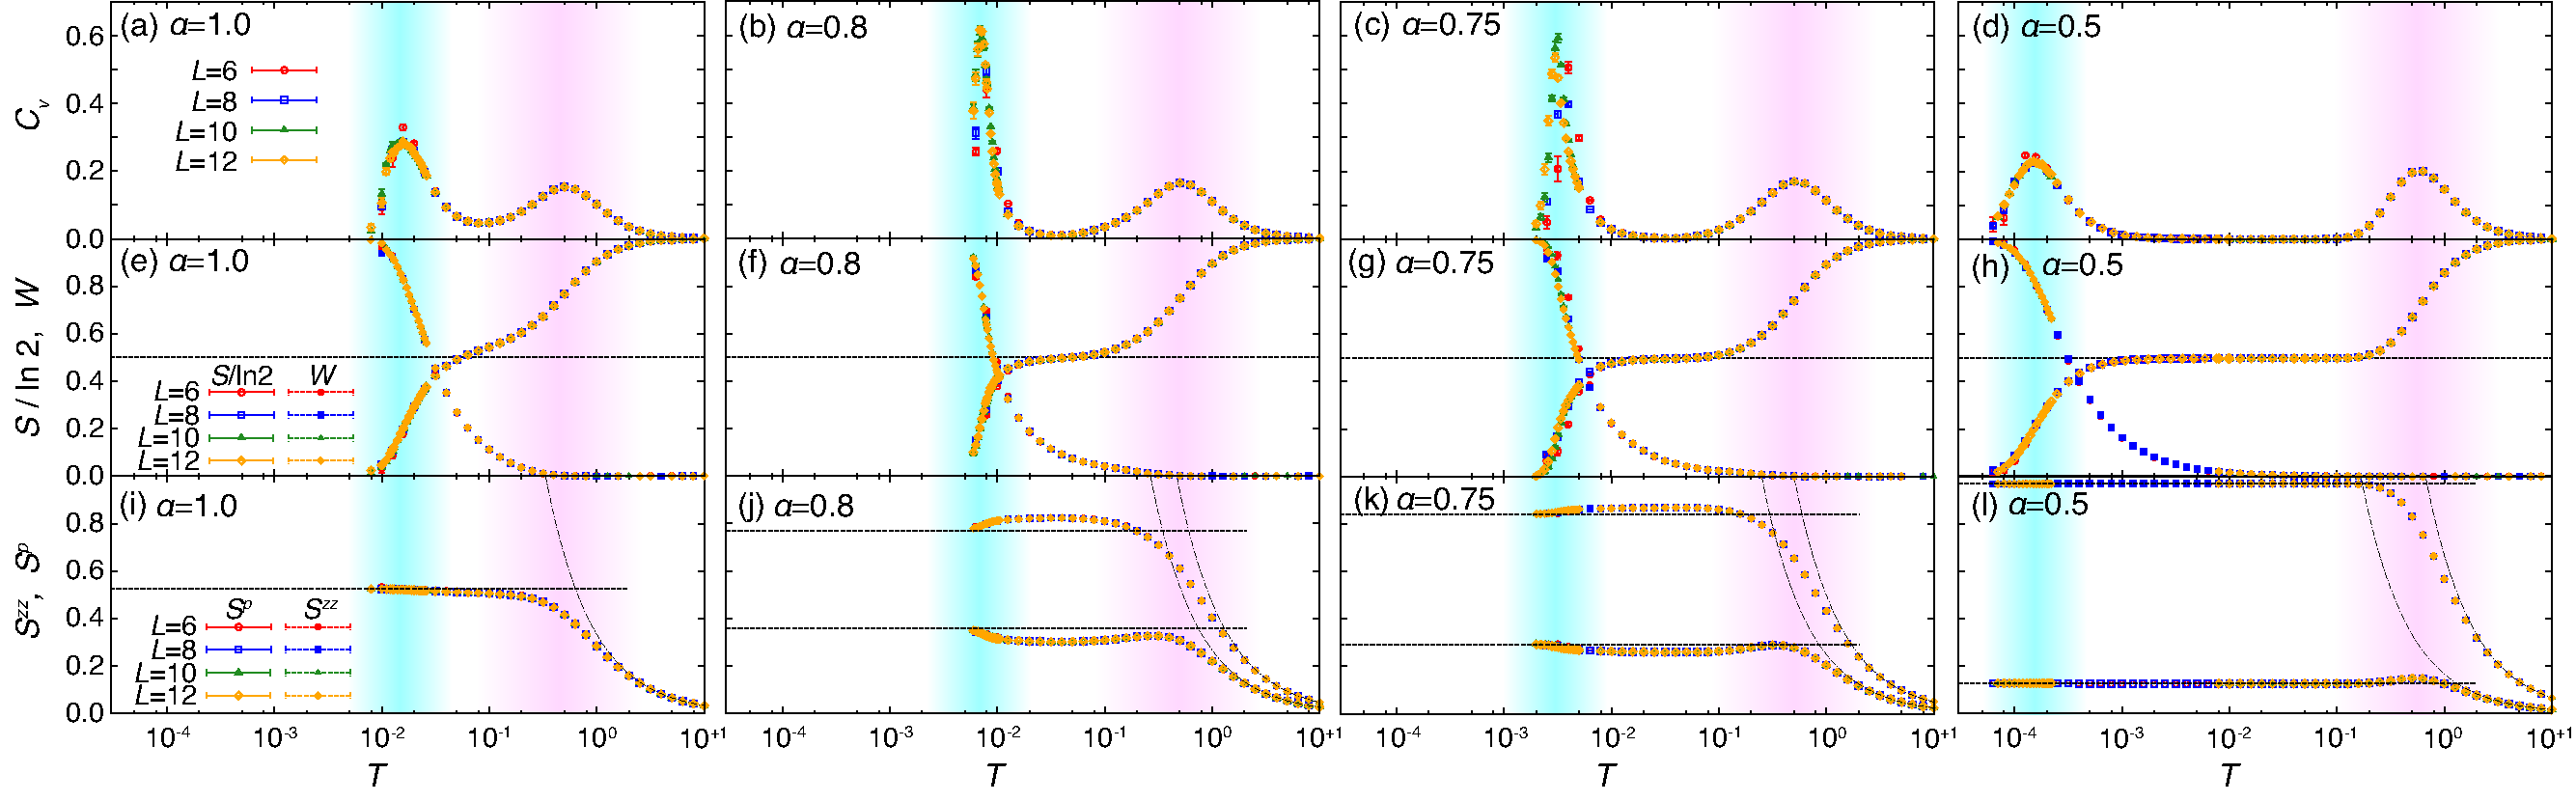
\includegraphics[width=\linewidth]{figures/Cv-eps-converted-to.pdf}
    \caption{Taken from Ref.~\cite{Nasu-Udagawa-Motome_2015}. According to the right-most figure, a sharp plateau appears in a specific temperature range when the system is in a \textbf{gapped phase}. The $\alpha$ is defined as a parameter that determines the ratio of the $J_x$ and $J_y$ couplings to the $J_z$. $J_x/J_z = J_y/J_z = \frac{\alpha}{3 - 2\alpha}$. By definition, the ratio of the exchange couplings is $J_x/J_z = J_y/J_z = 0.25$ if $\alpha = 0.5$, which is the situation of the right-most panel. \alert{\textbf{Question:} What will happen in the toric code limit?}}
    \label{fig:Cv}
\end{figure}

\begin{figure}
    \centering
    \includegraphics[width=0.3\linewidth]{alpha}
    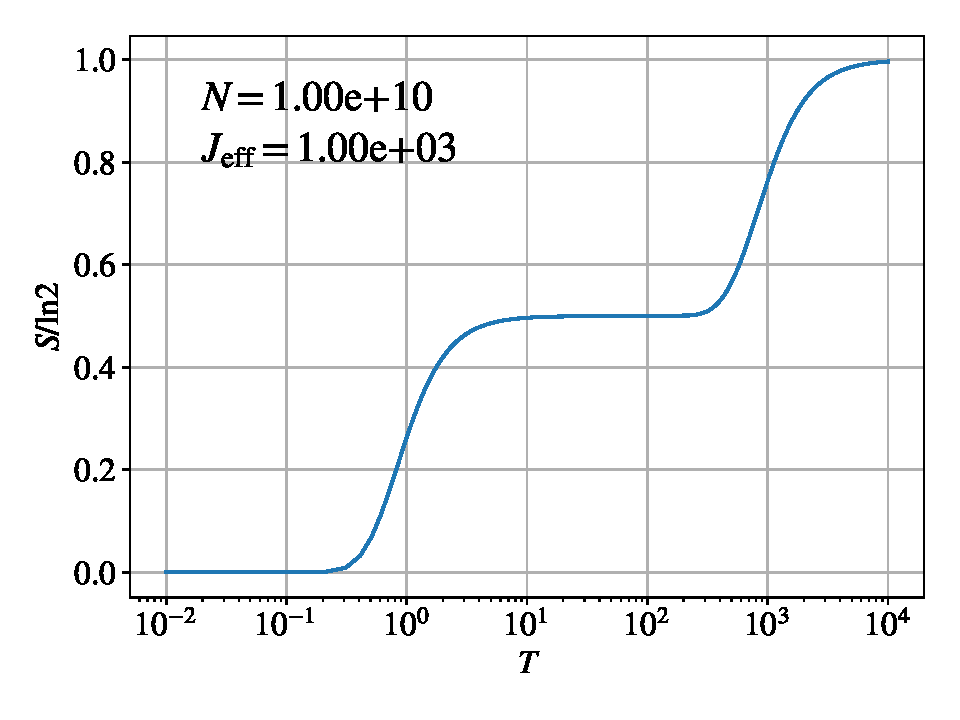
\includegraphics[width=0.3\linewidth]{figures/frac-sep-fig/J1000.pdf}
    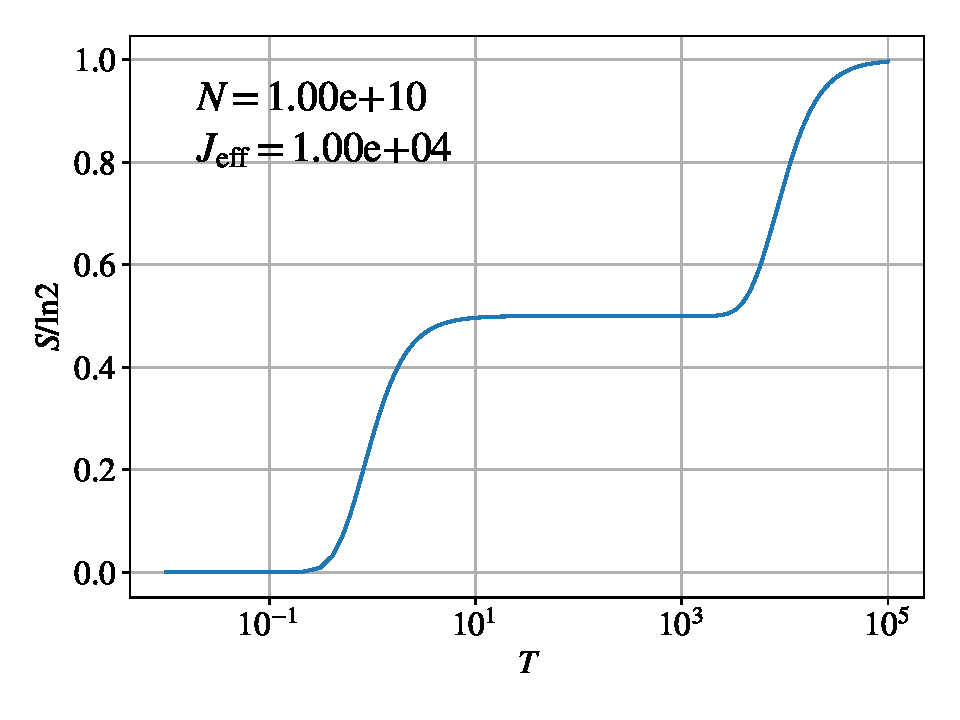
\includegraphics[width=0.3\linewidth]{figures/frac-sep-fig/J10000.pdf}
    \caption{The trend of thermal entropy per spin with temperature, calculated by definition $S = \ln Z - \beta\pdif{\beta}\ln Z$ directly. The system is the Kitaev model in the toric code limit. The size of the system is fixed to be $N = 10^{10}$, and $J_{\mrm{eff}}$ is the coupling constant of the low-energy effective theory appearing in Eq.~\eqref{eq:eff-model}. The \textit{melting point} of the static-flux phase does not depend on the value of $J_{\mrm{eff}}$. On the other hand, the \textit{melting point} of the free-spinon phase changes significantly when we vary $J_{\mrm{eff}}$. }
    \label{fig:entropy-sep}
\end{figure}


\appendix
%%%%%%%%%%%%%%%%%%%%%%%%%%%%%%%%%%%%%%%%%%%%%%%%%



\section{Exactly Solving for the Ground State}
According to equation (29) of Ref.~\cite{Kitaev_2006}, we can diagonalize the Kitaev Hamiltonian in the momentum space if the gauge is fixed to be $u_{ij} = +1\forall\; (ij)$, 
\[\hat{H} = \sum_{\bo{k}}\Psi^\dagger_{k}U(k)\Psi_{k} = \frac{1}{2}\sum_{\bo{k}}\lrm{is_{\bo{k}}d_{k,A}^\dagger d_{k,B} - is_{\bo{k}}^*d_{k,B}^\dagger d_{k,A}}\]
where
\[\Psi_k \equiv \frac{1}{\sqrt{2N}}\sum_{\bo{r}}e^{-ik\cdot \bo{r}}\begin{pmatrix}
                                                             c_{\bo{r},A} \\
                                                             c_{\bo{r},B}
                                                           \end{pmatrix} = \begin{pmatrix}
                                                                             d_{k,A} \\
                                                                             d_{k,B}
                                                                           \end{pmatrix}\]
\[U(k) = \frac{1}{2}\begin{pmatrix}
                      0 & is_{\bo{k}} \\
                      -is_{\bo{k}}^* & 0 
                    \end{pmatrix} \quad , \quad s_{\bo{k}} = 2\lr{J_xe^{ik\cdot \lr{\bo{a}_2 - \bo{a}_1}} + J_ye^{ik\cdot \bo{a}_2} + J_z}\]
Note that the index $\bo{r}$ above is the Bravais lattice point, and $A$,$B$ represent the sublattice. If we further define a normal fermion operator, 
\begin{equation}\label{gamm def.e}
  \gamma_{\bo{r}} \equiv \frac{1}{2}\lr{c_{{\bo{r}},A} + ic_{{\bo{r}},B}}
\end{equation}
 then its Fourier transform would be 
\[\gamma_{k} = \frac{1}{\sqrt{2N}}\sum_{{\bo{r}}}\gamma_{{\bo{r}}}e^{-ik\cdot \bo{r}} = \frac{1}{2}\lr{d_{k,A} + id_{k,B}}\]
In this way, the operator $d$ can be expressed in terms of $\gamma$ fermion,
\[
\left\{
\begin{aligned}
& d_{k,A} = \gamma_{-\bo{k}}^\dagger + \gamma_{k} \\
& d_{k,B} = i\lr{\gamma_{-\bo{k}}^\dagger - \gamma_{k}}
\end{aligned}
\right.
\]
Using the $\gamma$ operators to rewrite the Hamiltonian gives
\[\hat{H} = \sum_{\bo{k}}\lrm{R_\bo{k}\cdot\lr{\gamma_{\bo{k}}^\dagger \gamma_{\bo{k}} - \gamma_{-\bo{k}}\gamma_{-\bo{k}}^\dagger} - iI_\bo{k}\cdot\lr{\gamma_{k}^\dagger \gamma_{-\bo{k}}^\dagger - \gamma_{-\bo{k}}\gamma_{k}}} = \sum_{\bo{k}}\phi_k^\dagger\bo{H}(k)\phi_k\]
where $R_{\bo{k}} \equiv \mrm{Re}\lrg{s_{\bo{k}}}$ and $I_k \equiv \mrm{Im}\lrg{s_{\bo{k}}}$, and 
\[\bo{H}(k) \equiv \begin{pmatrix}
                R_{\bo{k}} & -iI_{\bo{k}} \\
                iI_k & -R_{\bo{k}} 
              \end{pmatrix} \quad,\quad \phi_k \equiv \begin{pmatrix}
                                                        \gamma_{\bo{k}} \\
                                                        \gamma_{-\bo{k}}^\dagger 
                                                      \end{pmatrix}\]
Since 
\[\bo{H}(k)^2 = \lr{R_{\bo{k}}^2 + I_k^2}\mathds{1} = \abs{s_{\bo{k}}}^2\mathds{1}\]
we can see that the eigenvalues are $\epsilon_{k} = \pm\abs{s_{\bo{k}}}$, which is consistent with Kitaev's result (equation (32) in Ref.\cite{KitaevOriginal}). To diagonalize the matrix $\bo{H}$ we have to apply the Bogoliubov transformation,
\begin{align*}
U &= \frac{1}{\sqrt{2\abs{s_{\bo{k}}}}}
        \begin{pmatrix}
           \mrm{sgn}(I_k)\sqrt{\abs{s_{\bo{k}}}+R_{\bo{k}}} & -i\sqrt{\abs{s_{\bo{k}}}-R_{\bo{k}}} \\
           i\sqrt{\abs{s_{\bo{k}}}-R_{\bo{k}}} & -\mrm{sgn}(I_k)\sqrt{\abs{s_{\bo{k}}}+R_{\bo{k}}} 
         \end{pmatrix} 
         = 
         \begin{pmatrix}
           \mrm{sgn}(I_k) u_k & -iv_k \\
           i v_k &  -\mrm{sgn}(I_k) u_k
         \end{pmatrix} \\
         &= 
         v_k\sigma^y + \mrm{sgn}(I_k)u_k\sigma^z
\end{align*}
such that\footnote{Those parameters in the matrix $U$ have the following properties: \textbf{(i)} $u_k = u_{-k}$, \textbf{(ii)} $v_{k} = v_{-k}$, and  \textbf{(iii)} $\mrm{sgn}(I_{k}) = -\mrm{sgn}(I_{-k})$} 
\[U\bo{H}U^\dagger = \begin{pmatrix}
                       \abs{s_{\bo{k}}} & 0 \\
                       0 & -\abs{s_{\bo{k}}} 
                     \end{pmatrix}\]
Therefore, the excitation that diagonalize the Hamiltonian is 
\begin{equation}\label{Bogo.e}
\begin{pmatrix}
    a_k \\
    a_{-k}^\dagger 
  \end{pmatrix} = U\begin{pmatrix}
                     \gamma_{\bo{k}} \\
                     \gamma^\dagger_{-k} 
                   \end{pmatrix} = \begin{pmatrix}
                                     \mrm{sgn}(I_k) u_k\gamma_{\bo{k}} - iv_k\gamma^\dagger_{-k} \\
                                     i v_k\gamma_{\bo{k}} - \mrm{sgn}(I_k) u_k\gamma^\dagger_{-k} 
                                   \end{pmatrix}
\end{equation}
As a result, the Kitaev ground state is the vacuum state of the Bogoliubov fermion, i.e., $a_{k}\ket{M} = 0$, which means $\ket{M}$ can be written as a BCS ground state just as we met in the BCS theory. The ground state can be written as the coherent state\footnote{
The coefficient $g_k$ can be represented in terms of $u_k$ and $v_k$. As I have mentioned, the BCS-like ground state is expected to be the vacuum state of $a_k$ fermions for all possible $k$, thus, we have
\[
\lr{\mrm{sgn}(I_k) u_k\gamma_{\bo{k}} - iv_k\gamma_{-\bo{k}}^\dagger}\prod_{k}\lr{\mathds{1} + g_k\gamma_{\bo{k}}^\dagger \gamma_{-\bo{k}}^\dagger}\ket{\vac_\gamma} = 0
\]
Based on this, we obtain that 
\[\mrm{sgn}(I_k) u_kg_k - iv_k = 0\]
therefore
\begin{equation}\label{g_k solution.e}
  g_k = \mrm{sgn}(I_k)i\frac{v_k}{u_k} = \mrm{sgn}(I_k) i\sqrt{\frac{\abs{s_{\bo{k}}} - R_{\bo{k}}}{\abs{s_{\bo{k}}} + R_{\bo{k}}}} = i\frac{\abs{s_{\bo{k}}} - R_{\bo{k}}}{I_k}
\end{equation}
} of the $\gamma$-fermion pair,
\begin{align*}
  \ket{M} &= A\lrm{g}\exp\lr{\sum_{\bo{k}}g_k \gamma^\dagger_k \gamma^\dagger_{-k}}\ket{\vac_\gamma}\\
   &= A\lrm{g}\exp\lr{\sum_{{\bo{r}}{\bo{r}'}}g_{{\bo{r}}{\bo{r}'}} \gamma^\dagger_{\bo{r}} \gamma^\dagger_{{\bo{r}'}}}\ket{\vac_\gamma}\\
   &= A\lrm{g}\lrm{\mathds{1} + \sum_{{\bo{r}}{\bo{r}'}}g_{{\bo{r}}{\bo{r}'}} \gamma^\dagger_{\bo{r}} \gamma^\dagger_{{\bo{r}'}} + \frac{1}{2!}\sum_{{\bo{r}}{\bo{r}'}\kappa\lambda}g_{{\bo{r}}{\bo{r}'}}g_{\kappa\lambda
   } \gamma^\dagger_{\bo{r}} \gamma^\dagger_{{\bo{r}'}}\gamma^\dagger_\kappa \gamma^\dagger_{\lambda} + \cdots}\ket{\vac_\gamma}
\end{align*}
where $\ket{\vac_\gamma}$ is the vacuum state of the $\gamma$-fermions, and $g_{{\bo{r}}{\bo{r}'}} = \frac{1}{2N}\sum_{\bo{k}}g_ke^{-ik\cdot(\bo{r}-\bo{r}')}$. 

\subsection{With External Magnetic Field}
For simplicity, we focus only on the isotropic limit~\cite{Kitaev_2006}. In this situation, applying an external magnetic field $\bo{h} = \lr{h_x,h_y,h_z}$, which is equivalent to adding a Zeeman perturbation $H' = -\sum_{i}\bo{h}\cdot\bog{\sigma}$, makes the Kitaev model equivalent to the Haldane honeycomb model~\cite{Haldane_1988} up to the third-order perturbation. The Hamiltonian under this approximation in the Majorana fermion representation reads
\begin{align*}
    H 
    &= 
    -\frac{1}{2}J\sum_{\bo{r}}
    \lr{
        ic_{\bo{r}A}c_{\bo{r}+\hat{\bo{n}}_1,B} 
        + 
        ic_{\bo{r}A}c_{\bo{r}+\hat{\bo{n}}_2,B}
        +
        ic_{\bo{r}A}c_{\bo{r}B}
        +\mrm{H.c.}
    } \\
    &\quad\quad\quad
    - 
    \frac{1}{2}\kappa
    \sum_{\bo{r}}\sum_{\mu = A,B}
    \lr{
        c_{\bo{r}\mu}c_{\bo{r}+\hat{\bo{n}}_1,\mu}
        +
        c_{\bo{r}\mu}c_{\bo{r}+\hat{\bo{n}}_2,\mu}
        +
        c_{\bo{r}\mu}c_{\bo{r}+\hat{\bo{n}}_1-\hat{\bo{n}}_2,\mu}
        +
        \mrm{H.c.}
    }
\end{align*}

\[
H = 
\frac{1}{2}
\sum_{\bo{k}}
\Psi_{\bo{k}}^\dagger
\begin{pmatrix}
  \Delta_{\bo{k}} & is_{\bo{k}} \\
  -is_{\bo{k}}^* & -\Delta_{\bo{k}}
\end{pmatrix}
\Psi_{\bo{k}}
\]
\[
\Delta_{\bo{k}} = 
\]

\section{Path Integrals for Majorana Fermions}
This note is based on the appendix of Ref.~\cite{Petrova-Mellado-Tchernychyov_2014} and Ref.~\cite{Shankar_2017}.

Consider a Hamiltonian represented in terms of Majorana fermions,
\[
H = \frac{1}{2} i \sum_{ij} c_i h_{ij} c_{j}
\]
where $c_i$ is the Majorana fermion mode satisfying the anti-commutation rule
\[
\lrg{c_i, c_j} = 2\delta_{ij}
\]
To find valid Grassman variables for Majorana fermions, we introduce redundant Majorana fermion modes $\lrg{\eta_i}$ that do not appear in the Hamiltonian and combine them with the physical Majorana modes $\lrg{c_i}$ to form normal fermion modes $\hat{\psi}_i = \frac{1}{2}\lr{c_i + i\eta_i}$. Substitution of the newly defined normal fermions into the Hamiltonian leads to
\[
H = \frac{i}{2} \sum_{ij} 
\lrm{\lr{\hat{\psi}_i + \hat{\psi}^\dagger_i} h_{ij} \lr{\hat{\psi}_j + \hat{\psi}^\dagger_j}}
\]
The corresponding coherent states and the Grassmann variables can be defined by

Grassmann integral for Majorana fermions can be defined in the usual way
\[
\int c\mrm{d}c = 2 \;,\; \int \mrm{d} c = 0
\]

\[
\int c\mrm{d} c = \int \lr{\psi + \bar{\psi}} \mrm{d} \lr{\psi + \bar{\psi}} = 2
\]


\section{Sum Rules for Correlation Functions}

\[
\rho 
= 
\frac{1}{2^{N-N_p}}
\mathcal{P}^{(p)}
\sum_{[\mathfrak{D}]}
\mathfrak{C}_{\mathfrak{D}}
\Sigma_{\mathfrak{D}}
\]
\[
\mathcal{P}^{(p)}
=
\lr{\frac{\mathds{1} + \tilde{W}_v}{2}}
\lr{\frac{\mathds{1} + \tilde{W}_h}{2}}
\prod_{p}\lr{\frac{\mathds{1} + W_p}{2}}
\]

\begin{align*}
    \rho^2 
    &= 
    \frac{1}{2^{2N-2N_p}}
    \mathcal{P}^{(p)}
    \sum_{[\mathfrak{D}]}\sum_{[\mathfrak{D}']}
    \mathfrak{C}_{\mathfrak{D}}
    \mathfrak{C}_{\mathfrak{D}'}
    \varphi(\mathfrak{D},\mathfrak{D}')
    \Sigma_{\mathfrak{D}\ominus\mathfrak{D}'}\\
    &=
    \frac{1}{2^{2N-2N_p}}
    \mathcal{P}^{(p)}
    \sum_{[\mathfrak{D}]}\sum_{[\mathfrak{D}']}
    \mathfrak{C}_{\mathfrak{D}}
    \mathfrak{C}_{\mathfrak{D}'}
    \frac{1}{2}
    \lrm{
    \varphi(\mathfrak{D},\mathfrak{D}')
    +
    \varphi(\mathfrak{D}',\mathfrak{D})
    }
    \Sigma_{\mathfrak{D}\ominus\mathfrak{D}'} \\
    &=
    \frac{1}{2^{2N-2N_p}}
    \mathcal{P}^{(p)}
    \sum_{[\mathfrak{D}]}\sum_{[\mathfrak{D}']}
    \mathfrak{C}_{\mathfrak{D}}
    \mathfrak{C}_{\mathfrak{D}'}
    \vartheta(\mathfrak{D},\mathfrak{D}')
    \Sigma_{\mathfrak{D}\ominus\mathfrak{D}'} \\
    &= 
    \frac{1}{2^{2N-2N_p}}
    \mathcal{P}^{(p)}
    \sum_{[\mathfrak{D}^c]}\sum_{[\mathfrak{D}']}
    \mathfrak{C}_{\mathfrak{D}^c\ominus\mathfrak{D}'}
    \mathfrak{C}_{\mathfrak{D}'}
    \vartheta(\mathfrak{D}^c\ominus\mathfrak{D}',\mathfrak{D}')
    \Sigma_{\mathfrak{D}^c} \\
    &=
    \frac{1}{2^{N-N_p}}
    \mathcal{P}^{(p)}
    \sum_{[\mathfrak{D}]}
    \lr{
        \frac{1}{2^{N-N_p}}
        \sum_{[\mathfrak{D}']}
        \mathfrak{C}_{\mathfrak{D}\ominus\mathfrak{D}'}
        \mathfrak{C}_{\mathfrak{D}'}
        \eta_{\mathfrak{D}'}
        \vartheta(\mathfrak{D},\mathfrak{D}')
    }
    \Sigma_{\mathfrak{D}}
\end{align*}

\begin{equation}\label{eq:strong-condition}
    \frac{1}{2^{N-N_p}}
    \sum_{[\mathfrak{D}']}
    \vartheta(\mathfrak{D},\mathfrak{D}')
    \mathfrak{C}_{\mathfrak{D}\ominus\mathfrak{D}'}
    \mathfrak{C}_{\mathfrak{D}'}
    =
    \mathfrak{C}_{\mathfrak{D}}
\end{equation}
\begin{equation}\label{eq:weak-condition}
    \frac{1}{2^{N-N_p}}
    \sum_{[\mathfrak{D}]}
    \mathfrak{C}_{\mathfrak{D}}^2
    =
    1
\end{equation}

notice that $\eta_{\mathfrak{D}}=1$ if $[\mathfrak{D}]\in \bo{G}$

\[
    \vartheta(\mathfrak{D},\mathfrak{D}') 
    = 
    \frac{1}{2}
    \lrm{
    1
    +
    \eta_{\mathfrak{D}}
    \eta_{\mathfrak{D}'}
    \eta_{\mathfrak{D}'\ominus\mathfrak{D}}
    }\varphi(\mathfrak{D},\mathfrak{D}')
    =
    \vartheta(\mathfrak{D}',\mathfrak{D})
    =
    \text{$0$ or $\pm 1$}
\]

\[
\varphi(\mathfrak{D}\ominus\mathfrak{D}',\mathfrak{D}') = \eta_{\mathfrak{D}}\eta_{\mathfrak{D}\ominus\mathfrak{D}'} \varphi(\mathfrak{D}',\mathfrak{D})
=
\eta_{\mathfrak{D}'} \varphi(\mathfrak{D},\mathfrak{D}')
\]

\[
\vartheta(\mathfrak{D}\ominus\mathfrak{D}',\mathfrak{D}')
=
\frac{1}{2}
\lrm{
    1
    +
    \eta_{\mathfrak{D}\ominus\mathfrak{D}'}
    \eta_{\mathfrak{D}'}
    \eta_{\mathfrak{D}}
}
\varphi(\mathfrak{D}\ominus\mathfrak{D}',\mathfrak{D}') 
= 
\eta_{\mathfrak{D}'}
\vartheta(\mathfrak{D},\mathfrak{D}')
\]

\begin{lemma}
    If $[\mathfrak{D}]\in\bo{G}$, then the following identity holds
    \[
    \sum_{[\mathfrak{D}']\in\bo{G}}\eta_{\mathfrak{D}\ominus\mathfrak{D}'} 
    = 
    \delta_{[\mathfrak{D}],[\varnothing]}
    \]
\end{lemma}
\begin{proof}
    By definition, the factor $\eta_{\mathfrak{D}}$ can be expressed as $\eta_{\mathfrak{D}} = (-1)^{\Delta(\mathfrak{D})/2}$, where $\Delta(\mathfrak{D}) \equiv n_a(\mathfrak{D})-n_b(\mathfrak{D})$. 
    \[
    \Delta(\mathfrak{D}\ominus\mathfrak{D}') 
    = 
    \Delta(\mathfrak{D})
    +
    \Delta(\mathfrak{D}')
    - n_a(\mathfrak{D}\cap\mathfrak{D}') 
    + n_b(\mathfrak{D}\cap\mathfrak{D}') 
    \]
    \[
    \eta_{\mathfrak{D}\ominus\mathfrak{D}'}
    =
    (-1)^{\Delta(\mathfrak{D}\ominus\mathfrak{D}')}
    =
    \eta_{\mathfrak{D}}\eta_{\mathfrak{D}'}
    (-1)^{n_a(\mathfrak{D}\cap\mathfrak{D}') }(-1)^{n_b(\mathfrak{D}\cap\mathfrak{D}')}
    =
    (-1)^{n_a(\mathfrak{D}\cap\mathfrak{D}') }(-1)^{n_b(\mathfrak{D}\cap\mathfrak{D}')}
    %(-1)^{ \abs{\mrm{EP}(\mathfrak{D}) \cap \mrm{EP}(\mathfrak{D}')} }
    \]
    \[
    \sum_{[\mathfrak{D}']\in\bo{G}} \eta_{\mathfrak{D}\ominus\mathfrak{D}'}
    =
    \sum_{[\mathfrak{D}']\in\bo{G}}(-1)^{n_a(\mathfrak{D}\cap\mathfrak{D}') }(-1)^{n_b(\mathfrak{D}\cap\mathfrak{D}')}
    \]
\end{proof}
\begin{lemma}
    If $[\mathfrak{D}]\in\bo{G}$, then the following identity holds
    \[
    \sum_{[\mathfrak{D}']\in\bo{G}} \Sigma_{\mathfrak{D}'}\Sigma_{\mathfrak{D}}\Sigma_{\mathfrak{D}'} 
    = 
    \delta_{[\mathfrak{D}],[\varnothing]}
    \mathds{1}
    \]
\end{lemma}
\begin{proof}
    According to the identity $\varphi(\mathfrak{D},\mathfrak{D}') = \eta_{\mathfrak{D}}\eta_{\mathfrak{D}'}\eta_{\mathfrak{D}\ominus\mathfrak{D}'}\varphi(\mathfrak{D}',\mathfrak{D})$, we have the commutation relation 
    \[
    \Sigma_{\mathfrak{D}}\Sigma_{\mathfrak{D}'} = \eta_{\mathfrak{D}\ominus\mathfrak{D}'} \Sigma_{\mathfrak{D}'}\Sigma_{\mathfrak{D}}
    \]
    In the above identity, we have already considered $[\mathfrak{D}],[\mathfrak{D}']\in\bo{G}$ in our case. With this relation, we could rewrite the summation in the equation we wanted to prove
    \[
    \sum_{[\mathfrak{D}']\in\bo{G}} \Sigma_{\mathfrak{D}'}\Sigma_{\mathfrak{D}}\Sigma_{\mathfrak{D}'}
    =
    \sum_{[\mathfrak{D}']\in\bo{G}} 
    \eta_{\mathfrak{D}\ominus\mathfrak{D}'}
    \Sigma_{\mathfrak{D}}
    \]
\end{proof}

%\section{blank}

\bibliographystyle{my_apsrev4-2}
\bibliography{ref}% Produces the bibliography via BibTeX.




\end{document} 